\documentclass[letterpaper,twocolumn,10pt]{article}

\usepackage[utf8]{inputenc}
\usepackage{usenix}
\usepackage[top=2cm,bottom=2.5cm,left=2cm,right=2cm]{geometry}
\usepackage{balance}
\usepackage{tikz}
\usepackage{xspace} % For reasonable spacing in custom commands.
\usepackage{xcolor} % For colourful links.
\usepackage[backend=biber,backref=true,maxnames=20,urldate=long]{biblatex}
\usepackage{hyperref} % For clickable links.
\usepackage[l2tabu, orthodox]{nag}
\usepackage{subcaption}
\usepackage{booktabs}
\usepackage{enumitem} % For custom symbols in enumerations.
\usepackage{wasysym}  % For \Square and \Circle.
\usepackage[english]{babel}
\usepackage{csquotes}

\usepackage[T1]{fontenc}
\usepackage[scaled=0.8]{beramono}
\usepackage[scaled=0.8]{berasans}

\urlstyle{sf}

\setlength{\columnsep}{0.7CM}

\addbibresource{paper.bib}

\definecolor{darkblue}{rgb}{0.1,0.1,0.4}

\usetikzlibrary{positioning}

\newcommand{\ie}{\textit{i.e.}\xspace}
\newcommand{\eg}{\textit{e.g.}\xspace}
\newcommand{\ea}{\textit{et al.}\xspace}
\newcommand{\etc}{\textit{etc.}\xspace}
\newcommand{\aka}{a.k.a.\xspace}
\newcommand{\first}{(\textit{i})\xspace}
\newcommand{\second}{(\textit{ii})\xspace}
\newcommand{\third}{(\textit{iii})\xspace}
\newcommand{\fourth}{(\textit{iv})\xspace}
\newcommand{\fifth}{(\textit{v})\xspace}

\hypersetup{
	pdftitle={How do Tor users interact with onion services?},
	pdfauthor={},
	pdfkeywords={},
	colorlinks=true,
	urlcolor=darkblue,
	linkcolor=darkblue,
	citecolor=darkblue
}

\renewcommand*{\bibfont}{\small}

\begin{document}

% Don't want date printed
\date{}

\title{
    {\Large \textbf{How do Tor users interact with onion services?}}
}

\author{}

\maketitle

% Use the following at camera-ready time to suppress page numbers.
% Comment it out when you first submit the paper for review.
\thispagestyle{empty}

\subsection*{Abstract}
% Problem statement.
Onion services are anonymous TCP services that are only accessible over the Tor
network.  As of November 2017 more than 50,000 onion services provide anonymous
web sites, chat protocols, and file sharing services.  This surge in popularity
brought with it a Wild West of phishing attacks and scams, countered by ad-hoc
countermeasures and usability improvements.  These countermeasures have in
common that they have not been formally studied.
% What we are doing.
In this work we fill this gap by studying how people perceive, understand, and
use onion services.  To that end we employ a mixed-methods approach consisting
of semi-structured interviews to explore the problem space, and an online
survey to solicit answers to concrete questions.  We find that users place great
trust in The Tor Project but distrust content that is hosted on onion services.
Users have devised a diverset set of methods to work around the non-memorable
domain format.
% Why our work matters.
Our work enables privacy engineers---in particular Tor developers---to improve
their technology.


\section{Introduction}
\label{sec:introduction}

The colloquial meaning behind online anonymity implies \emph{client anonymity},
\ie, a user disguises her IP address, for example by using a VPN.  A
lesser-known use case is \emph{server anonymity} which allows a web service to
disguise its IP address.  Service operators have good reasons to employ server
anonymity; be it to escape harassment, speak out against power, or voice
dissenting opinions.  Tor's onion services provide what may be the most popular
way of running an anonymous TCP service.\footnote{Onion services used to be
known as ``hidden services'' but were recently renamed to reflect the fact
that onion services provide more than just ``hiding'' a service---most
importantly end-to-end security and self-authenticating names.}

Originally deployed in 2004, onion services have grown substantially over the
last years, both in the number of services and users.  As of January 2018, The
Tor Project's statistics count more than 60,000 onion services each day,
relaying an aggregate of more than 750 Mbps of network traffic.  Not all of
these services host web sites; use cases such as metadata-free instant
messaging~\cite{ricochet} and file sharing~\cite{onionshare} have emerged as
well.  The Tor Project currently does not have information on the number of
onion service users but Facebook reported in 2016 that more than one million
users logged into their onion service over a one-month
period~\cite{facebook-users}.

Regarding usability, onion services differ from conventional web services in
several aspects; \first they can only be accessed over the Tor network; \second
their domain is a hash over their public key, rendering them hard to remember;
\third network latency is noticeable because of the additional hops in between
client and onion service; and \fourth onion services are private by default,
requiring manual dissemination.  To date our understanding of how users deal
with these idiosyncrasies is anecdotal.  We fill this gap by studying how Tor
users interact with onion services.  In particular, we set out to understand
users' mental model of Tor, their expectations of privacy, issues that they
experience, and how they adapted their workflows to deal with onion services.

Onion services do not exist in a vacuum.  They are tightly coupled to their
surrounding software ecosystem---most importantly Tor Browser---which is why an
isolated study of onion services is bound to miss important context.  While our
research question is about onion services, we aim to get as complete a picture
as possible by casting a wider net and answering open questions about the use of
Tor Browser in particular and privacy expectations in general.  To that end we
employ a mixed-methods approach involving the creation of an online survey that
asked participants to answer an array of questions on Tor Browser, onion service
usage and operation, onion site phishing, and general expectations of privacy.
Based on our survey questions, our interviews let us ask follow-up questions and
dive deeper into unexpected answers.

Our most salient findings show that \first the flawed mental model some users
have of Tor may cause security issues such as a blind reliance on vanity onion
domains, \second the domain format of onion services, while cumbersome, is not
among the most pressing usability issues, \third the content that onion services
are perceived to host causes trust issues for non-technical users, and \fourth
onion service operators seek to foil phishing attacks by having devised a number
of strategies, many of which are ineffective.

At the time of this writing, The Tor Project is testing the next generation of
onion services, intended to fix security issues and transition to faster and
future-proof cryptography.  We hope that our results can inform this process.
Finally, since many of our findings touch on various aspects of privacy and
anonymity, we believe that privacy tools other than Tor, \eg I2P, can benefit
from our findings.  In summary, we make the following contributions:

\begin{itemize}
    \item We interviewed seventeen Tor users of diverse backgrounds to
        understand their habits, assumptions, and expectations related to Tor.
        Using qualitative data coding, we identified novel themes that underlay
        our interview data.

    \item We administered an online survey for Tor users, reaching 621 people.
        Our survey focused on the most salient issues around onion services,
        \eg, the domain format, onion service discovery, and phishing attacks.

    \item Drawing on our two datasets, we identify \first incorrect mental
        models, \second key issues that impede the adoption and use of onion
        services, and \third ways forward to improve onion services.
\end{itemize}

The rest of this paper is structured as follows.  We begin by discussing related
work in Section~\ref{sec:related-work}, followed by background on onion services
in Section~\ref{sec:background}.  Section~\ref{sec:method} then presents the
methods we used for our interviews and online survey, followed by
Section~\ref{sec:results} which discusses our findings from both data sources.
Finally, we discuss our results in Section~\ref{sec:discussion} and conclude our
work in Section~\ref{sec:conclusion}.


\section{Related Work}
\label{sec:related-work}

The usability of Tor Browser has seen numerous substantial changes since its
creation in 2003~\cite{Syverson2005a}; from a manually-installed Tor ``button,''
to the Tor Browser Bundle, and to the currently-used Tor Browser, installation was
not always as easy as it is today. Indeed, the installation woes of yesteryear
prompted Clark, van Oorschot, and Adams 
to use cognitive walkthroughs to study how users install, configure, and run
Tor Browser~\cite{Clark2007a}.  The authors uncovered usability hurdles such as
jargon-laden documentation, confusing menus, and insufficient visual feedback.
As of February 2018, the study is ten years old, and Tor Browser has undergone
radical changes in this time.

More recently, in 2014 Norcie \ea\ identified stop-points in the
installation and use of the Tor Browser Bundle~\cite{Norcie2014a}.\footnote{The
Tor Browser Bundle was later rebranded and is now known as Tor Browser.}  These
stop-points represent places in a user interface that require action but are met
instead with confusion by users.  Having identified these stop-points, the
authors then issued interface design recommendations and subsequently tested
these recommendations in a user study.

Inspired by Tor Browser's use as an anti-censorship system, Fifield \ea\ published
a design to study its usability as a censorship circumvention
tool~\cite{Fifield2015a}.  Drawing upon both qualitative and quantitative
methods, the authors plan on recruiting hundreds of users to study how they use Tor
Browser's configuration wizard in an adversarial setting.  Lee
\ea~\cite{Lee2017a} studied the usability of Tor Launcher, the graphical
configuration tool that allows users to configure Tor Browser.  Their findings
paint a bleak picture: 79\% of users' connection attempts in a simulated
censored environment failed.  However, the researchers showed that their
proposed interface improvements resulted in less difficulties for users.

Forte \ea\ studied the privacy practices of contributors to open collaboration
projects~\cite{Forte2017a}.  The authors interviewed 23 contributors to The Tor
Project and Wikipedia to learn about how privacy concerns affect their
contribution practices.  The study found that contributors worry about an array
of threats including surveillance, violence, harassment, and loss of
opportunity.

Most recently in 2017, Gallagher \ea\ conducted a series of semi-structured
interviews to understand both why people use Tor Browser and how they understand
the technology~\cite{Gallagher2017a}.  The authors found that experts tend to
have a network-centric view of the Tor network and tend to use it frequently
while non-experts have a goal-oriented view and see Tor Browser as a black box
that provides a service.  Our own work supports these findings.  Consequently,
non-experts do not use Tor Browser if they do not need its service.
Furthermore, non-experts tend to consider a single threat while the threat model
of experts contains multiple actors.

Several research efforts sought to alleviate the handling of randomly-generated
domain names.  Sai and Fink proposed a mnemonic system that maps 80-bit onion
domains to sentences~\cite{Sai2012a}.  Their work is inspired by mnemonicode, a
method to map binary data to words~\cite{mnemonicode}.  Victors \ea\ proposed a
more radical approach by designing the Onion Name System~\cite{Victors2017a}
which allows users to reference an onion service by a meaningful and
globally-unique identifier.  Kadianakis \ea\ designed a modular name system
\textsc{api} that allows Tor clients to configure name systems (\eg,
\textsc{gns}~\cite{Schanzenbach2012a} or OnioNS~\cite{Victors2017a}) on a
per-domain basis~\cite{Kadianakis2016a}.  Kadianakis summarized the current
state of research on onion service naming systems in a blog
post~\cite{Kadianakis2017a}.

We improve on the existing body of work by studying unanswered questions about
the use of Tor Browser and---the focus of this paper---how users interact with
onion services.  We believe that some of our findings generalize to other
systems, \eg, Freenet~\cite{Freenet} and Bitcoin~\cite{Nakamoto2008a} also
employ self-authenticating names---Freenet in its file naming scheme and Bitcoin
in its addressing scheme.


\section{Background}
\label{sec:background}

Onion services are TCP services that are only accessible over the Tor network.
While conventional Internet services are contacted over their IP address, onion
services are contacted over their onion domain, which is resolved and routed
inside the Tor network.  Due to onion services being hosted in the Tor network,
network traffic traverses six Tor relays (see Figure~\ref{fig:onion-service})
before it reaches the onion service.  The resulting increase in latency is the
cost of the anonymity that onion services provide.

\begin{figure*}[ht]
\centering
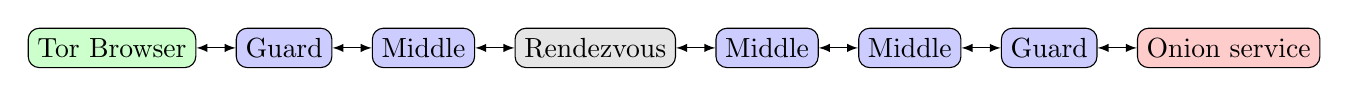
\begin{tikzpicture}[node distance=0.5cm]
\tikzset{>=latex}

\tikzstyle{block} = [rectangle, draw, rounded corners, text centered,
                     minimum height=0.5cm]

\node[block,fill=green!20]             (TB)  {Tor Browser};
\node[block,fill=blue!20,right=of TB]  (GR1) {Guard};
\node[block,fill=blue!20,right=of GR1] (MR1) {Middle};
\node[block,fill=gray!20,right=of MR1] (R)   {Rendezvous};
\node[block,fill=blue!20,right=of R]   (MR2) {Middle};
\node[block,fill=blue!20,right=of MR2] (MR3) {Middle};
\node[block,fill=blue!20,right=of MR3] (GR2) {Guard};
\node[block,fill=red!20,right=of GR2]  (OS)  {Onion service};

\draw[<->] (TB.east)  -- (GR1.west);
\draw[<->] (GR1.east) -- (MR1.west);
\draw[<->] (MR1.east) -- (R.west);
\draw[<->] (R.east)   -- (MR2.west);
\draw[<->] (MR2.east) -- (MR3.west);
\draw[<->] (MR3.east) -- (GR2.west);
\draw[<->] (GR2.east) -- (OS.west);

\end{tikzpicture}
\caption{When a user connects to an onion service, there are six relays in
between her Tor Browser (on the left) and the onion service (on the right).}
\label{fig:onion-service}
\end{figure*}

To create an onion domain, a Tor client first generates an RSA key pair.  It
then computes the SHA-1 hash over the RSA public key, truncates it to 80 bits,
and encodes these 80 bits in Base32, resulting in sixteen characters, \eg,
\texttt{expyuzz4wqqyqhjn}.  Due to the domain being a function of the public
key, onion domains are self-authenticating, meaning that as long as a client has
the correct domain, it knows what public key to expect.  The downside is that
sixteen random characters are impractical to remember.  However, onion domains
can be made at least partially meaningful by repeatedly creating RSA keys until
the resulting domain contains a desired string.  These domains are referred to
as \emph{vanity onion domains}.  The longer the desired string, the more time it
takes to find a matching key pair.  In practice, onion service operators use
tools such as scallion~\cite{scallion} that parallelize the search for suitable
keys to speed up the process.  Vanity domains are used by several organizations
such as Facebook (\url{facebookcorewwwi.onion}), ProPublica
(\url{propub3r6espa33w.onion}), and the New York Times
(\url{nytimes3xbfgragh.onion}).

Onion services are private by default.  Once an onion service is created, it is
up to its operator to announce it to the public, \eg, by adding it to onion site
search engines such as Ahmia.\footnote{The search engine is available online at
\url{https://ahmia.fi}.}  The lack of a go-to service such as Google for
onion service discovery means that the community has devised various ways to
publish onion services; most importantly an array of search engines and curated
lists.


\section{Interviews}
\label{sec:interviews}

We conducted a series of semi-structured interviews on the use of Tor Browser
and onion services to \first explore user experience outside the constraints of
an online survey and to \second inform the creation of our survey---and vice
versa because we conducted some interviews after our survey ended.

\subsection{Method}

We developed a question set that served as the basis for each
interview.\footnote{The question set is available online at
\url{https://nymity.ch/onion-services/pdf/interview-checklist.pdf}.}  The
semi-structured nature of our interviews allowed us to deviate from this
question set, \eg, by asking follow-up questions.  We began by asking
demographic information (gender, age range, occupation, country of residence,
and level of education), followed by information about online behavior, and
finally questions specific to Tor Browser and onion services.

\subsubsection{Recruitment}

To select eligible interview subjects, we created a short pre-interview survey
(see Appendix~\ref{sec:interview-survey}), which was advertised by The Tor
Project both in a blog post~\cite{Winter2017a} and on its Twitter account.  Our
selection process favored laypeople and sought to maximize cultural, gender,
location, education, and age diversity.  In addition to our online screening, we
recruited participants in person at an Internet freedom event.  We found it
difficult to draw a uniform sample of Tor users to interview. We believe that
The Tor Project's blog and Twitter account are mainly followed by
disproportionately technical users while many non-technical users may install
Tor Browser in a one-off process and then cease to follow the project.  To make
matters worse, many Tor users value their privacy significantly more than the
average Internet user, making it challenging to evoke enough trust to have users
open up to us about their browsing habits.

We ended up interviewing seventeen subjects whose demographic information is
shown in Table~\ref{tab:interviewees}.  Given the sensitive nature of our
interviews, we only present aggregate information to protect the identity of our
participants.  We believe that our sample is biased towards educated and
technical users (almost 60\% of our participants have a postgraduate degree) but
it also shows the diversity among Tor's user base: Our participants comprised
human rights activists, legal professionals, writers, artists, and journalists,
just to name a few.

\begin{table*}[ht]
	\centering
	\begin{tabular}{l r r | l r r | l r r | l r r}
	\toprule
	Age & \# & \% &
	Gender & \# & \% &
	Continent of residence & \# & \% &
	Education & \# & \% \\
	\midrule
	18--25 & 2  & 11.8 & Female & 5  & 29.4 & Asia          & 3 & 17.6 & No degree    & 1  & 5.9 \\
	26--35 & 10 & 58.8 & Male   & 12 & 70.6 & Australia     & 1 &  5.9 & High school  & 3  & 17.7 \\
	36--45 & 4  & 23.5 &        &    &      & Europe        & 4 & 23.5 & Graduate     & 3  & 17.7 \\
	46--55 & 1  & 5.9  &        &    &      & North America & 8 & 47.1 & Postgraduate & 10 & 58.8 \\
	       &    &      &        &    &      & South America & 1 &  5.9 & & & \\
	\bottomrule
	\end{tabular}
	\caption{The distribution over gender, age, country of residence, and
	education for our seventeen interview subjects.  We chose not to display
	per-person demographic information to protect the identity of our interview
	subjects.}
	\label{tab:interviewees}
\end{table*}

\subsubsection{Procedure}

Princeton University's institutional review board (IRB) deemed our study exempt
from further review.\footnote{Our IRB protocol number is 8251.}  We conducted
thirteen interviews in person and four interviews remotely; over Skype, Signal,
WhatsApp, and Jitsi---depending on what our interviewees felt the most
comfortable with.  For in-person interviews we asked our interviewees to sign a
consent form.  This was not practical for remote interviews, so we sent the
consent form in advance over email and, after seeking permission from our IRB,
asked for verbal consent before the interview.  In all cases we explicitly asked
for permission to record the conversation.  All except two participants agreed
to have their interview recorded.  In the remaining two interviews we took notes
instead.  We made it clear to our participants that they could withdraw their
consent at any time.  Each interview ended with a debriefing phase in which we
asked if our participants had any remaining questions.  Some wanted to know if
technical explanations they provided earlier were correct.  Finally, we offered
our participants a gift card worth twenty dollars as a token of appreciation.

We used the services of the company Rev to have our recordings transcribed.  A
mutually-signed non-disclosure agreement protected the confidentiality of our
data.  Once our our interview recordings were transcribed, we deleted the
original recordings and employed qualitative data coding to analyze the
transcripts.  Each interview transcript was coded by two members of our team.
This process identified twenty-seven themes that are all listed in
Appendix~\ref{sec:coding-themes}.

\subsection{Results}

We now discuss how our interview participants \emph{use}, \emph{perceive}, and
\emph{(mis)understand} both Tor and onion services.

\subsubsection{Understanding}

\begin{figure}[t]
    \centering
    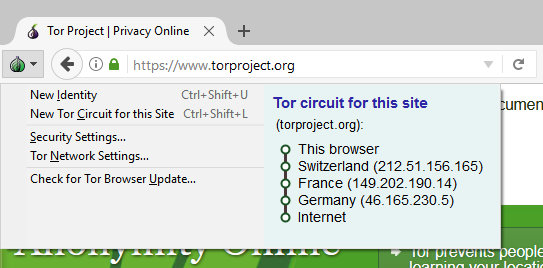
\includegraphics[width=\linewidth]{figures/tor-button-screenshot.jpg}
    \caption{A click on the onion icon reveals the Tor relays that constitute
    the circuit that was used to fetch the current page.}
    \label{fig:tor-button}
\end{figure}

Several of our participants enjoyed the visual feedback in Tor Browser (see
Figure~\ref{fig:tor-button}) that shows the circuit that is used for a given
site.  One interviewee mentioned:

\begin{displayquote}
I love how I can monitor the network through this little kind of bar that comes
up.
\end{displayquote}

Not satisfied with only seeing the current circuit, some participants wished it
were easier to learn what else is happening behind the scenes:

\begin{displayquote}
{[It]} would be nice to have some kind of application, something on that browser,
that gives you an impression of\dots what the Tor Browser's actually doing.
\end{displayquote}

Finding the right balance between what information to show and what to hide is
challenging by itself, and only exacerbated by Tor's technically diverse user
base.  While technical users may appreciate a closer look ``under the hood,''
non-technical users, who often see Tor as a tool to get a specific job
done~\cite[\S~4.3.2]{Gallagher2017a}, can easily feel bewildered and
overwhelmed.  One aspect in which more transparency could benefit Tor's entire
user base is when sites don't load:

\begin{displayquote}
\dots maybe some sort of graphical representation of is the circuit still
being built, or is the circuit built, and the site isn't responding at all to
the third relay?
\end{displayquote}

A comprehensible feature is an indicator of the anonymity that Tor Browser can
provide in a given situation:

\begin{displayquote}
In terms of the anonymity, you can't really tell\dots That's fairly opaque, so I
can't even tell how effective that's working, or whether it is\dots
\end{displayquote}

Quantifying anonymity in a real-world setting is complex, error-prone, and often
misleading.  What's more, Tor Browser does not have available all the data it
would need to quantify its user's anonymity, \eg, intermediate autonomous
systems, personal threat models, or the number of users that browse through Tor
in the same autonomous system.  For these reasons an ``anonymity meter'' is
likely a dead end, which is why The Tor Project focuses its efforts on
documentation and education.  Having been exposed to some of this documentation,
some of our participants lamented its limitations.  Asked about the difficulties
of setting up an onion service, one participant responded:

\begin{displayquote}
Tor does a good job on their web site of telling you to modify your
[configuration] file, and then getting the onion set up.  But it's just very
basic.  I have to go [to] other people's blog post to find out.
\end{displayquote}

Comprehensive documentation is only useful if it is understood.  One participant
struggled with the lack of localization.  While Tor Browser's user interface is
available in Spanish, the documentation is not:

\begin{displayquote}
Think more [about] the Spanish community\dots because in my case I'm trying to
train people to use Tor but I work in the indigenous communities and there are
some things that [are] hard for me to explain in terms of how you use Tor\dots
\end{displayquote}

\subsubsection{Misunderstandings}

We asked our participants to draw sketches of how they believe Tor and onion
services work.\footnote{All sketches are available online at
\url{https://nymity.ch/onion-services/mental-models/}.}   Everybody drew a
sketch of Tor but some didn't draw onion services because they had no mental
model for it.  Interestingly, all participants understood that bouncing network
traffic across several relays is key to Tor's anonymity, as evidenced by
Figure~\ref{fig:tor-sketch} which stems from a participant with no technical
background. Note that some details of the sketch are incorrect.  Tor uses
three-hop circuits and circuits the forward and reverse path are the same.
Analogously, most of our participants understood that network traffic does not
leave the Tor network when connecting to onion services.
Figure~\ref{fig:os-sketch} illustrates an example, again drawn by a
non-technical participant.

\begin{figure}[t]
    \centering

    \begin{subfigure}[t]{\linewidth}
        \centering
        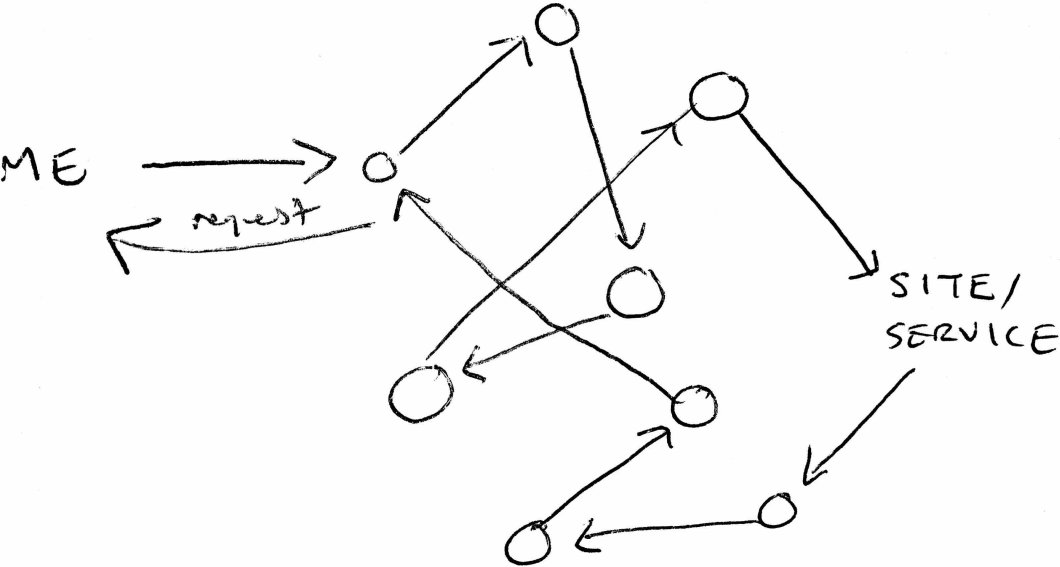
\includegraphics[width=0.8\linewidth]{figures/tor-sketch.jpg}
        \subcaption{A non-technical interview subject's sketch of how they
        believe Tor works.  The participant correctly understands the concept of
        bouncing network traffic over several hops.}
        \label{fig:tor-sketch}
    \end{subfigure}

    \begin{subfigure}[t]{\linewidth}
        \centering
        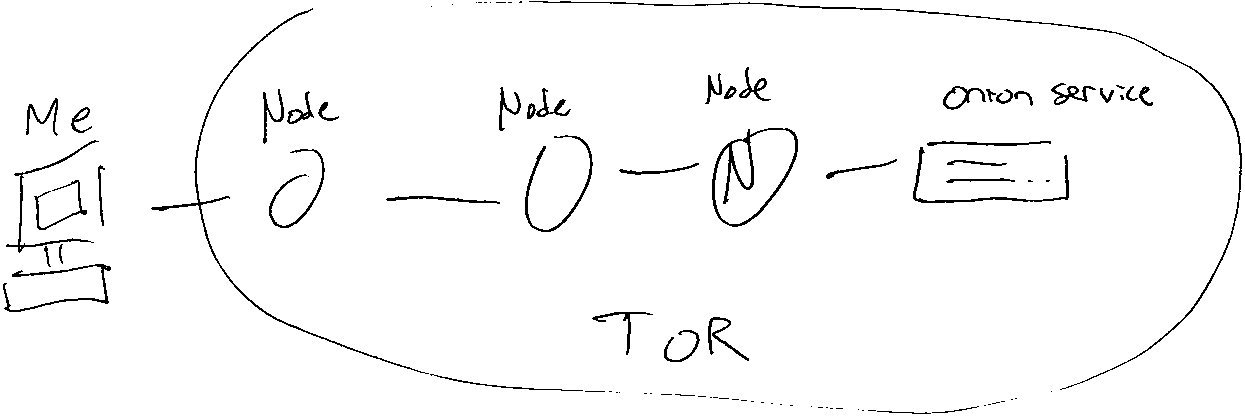
\includegraphics[width=0.8\linewidth]{figures/os-sketch.jpg}
        \subcaption{A non-technical interview subject's sketch of their mental
        model of an onion service.  Instead of a web site, the final hop is
        another Tor hop.}
        \label{fig:os-sketch}
    \end{subfigure}

    \caption{Sketches of two different, non-technical interview participants of
    how Tor works (top) and how onion services work (bottom).}
\end{figure}

Some of our interviewees did not distinguish disguising their IP address from
disguising their real-world identity, and instead used the umbrella term of
``anonymity'' to refer to both concepts.  This conflation of concepts paints an
incomplete picture of the security and privacy guarantees that Tor can provide,
as evidenced by one participant:

\begin{displayquote}
What's the point of going to Facebook using onion services when their business
model is still about collecting your data?
\end{displayquote}

There is still merit in using Facebook's onion service.  While the company
indeed learns who is logging in, they will not learn their users' location and
operating system, and users get end-to-end security outside of the often brittle
X.509 ecosystem as well as self-authenticating names.  These benefits are
difficult to convey if users don't understand the nuances in online anonymity.
Even technical users sometimes exhibit this ``all or nothing'' approach to
anonymity.

An unrelated yet hardly unexpected source of confusion is the domain format of
onion services.  Some users have come to believe that the seemingly-random
characters in onion domains is the reason why onion services are anonymous.
Accordingly, these users also believe that vanity domains are ``less anonymous''
because part of their domains is clearly not random.

\subsubsection{Perception}

Public perception of The Tor Project and the work it does is heavily tied to
adoption.  Among our interview participants, The Tor Project enjoyed a lot
of trust:

\begin{displayquote}
Because, you guys\dots have the sort of\dots not a monopoly on trust, but you
have like a really great brand name when it comes to this stuff\dots
\end{displayquote}

Upon being told what an onion service is, one participant responded:

\begin{displayquote}
So it's like the Hidden Wiki and stuff like that, where you can buy drugs
and\dots or supposedly.
\end{displayquote}

Crime taking place over Tor and particularly on onion services was a common
theme.  Most of our participants feel safer when using Tor Browser instead of
another browser.  Some further distinguished between security and privacy, with
one respondent saying that ``\emph{Mozilla and Google do a lot for security but
    not for privacy}.''  Another participant 

\subsubsection{Disadvantages}

We were particularly interested in hearing what kind of issues Tor users face.
Perhaps the most common issue is (still) browsing speed:

\begin{displayquote}
The speed of it is problematic; sometimes I have a path that allows me to watch
streaming full HD YouTube videos, and the next time five minutes later I'm
barely getting kilobytes through.
\end{displayquote}

Occasionally, Tor's reputation precedes it and prepares users for what to
expect:

\begin{displayquote}
I didn't think it was as slow as people say it was. People said it would be much
slower experience but\ldots a little bit slower, but it didn't matter for the
things that I was doing.
\end{displayquote}

In addition to the perceived slowness, several participants lamented the
old-fashioned user interface.  Tor Browser's looks were described as
``\dots\emph{it felt like it was about five years outdated},'' ``\dots\emph{it
looked like I was in 1982},'' and ``\emph{I think the colors look a bit old
fashioned and in the former Soviet Union}\dots''

Many of our participants expressed concern that their use of Tor makes them
``stick out'' or paints a target on their backs.  Asked about the disadvantages
of using Tor, one participant responded:

\begin{displayquote}
The fact that you're using Tor.  So I think that alone to [an]\dots experienced
observer might be cause in some countries to ring your doorbell and ask what
you're up to.
\end{displayquote}

Another participant expressed this concern for other privacy tools as well:

\begin{displayquote}
When you have it on your laptop, for some authorities, that is a reason to think
of you as somebody who's deserving of suspicion.  Same thing when you have
Signal, or when you use PGP, just by having [these] that means that they
sometimes are inclined to think that, ``Oh you must have something to hide
because you've used these kind of technologies.''
\end{displayquote}

Interestingly, one participant expressed that the antiquated user interface
evoked trust:

\begin{displayquote}
At the same time I thought I think that it gave them a certain amount of
credibility, like they weren't building this for the looks, but they were
building it for functionality, so what it did.  At the same time, as I thought
it was outdated in terms of how it looked, I also thought it was sort of genuine
in a way.
\end{displayquote}

In 2016, Khattak \ea documented how Tor users are often treated differently than
non-Tor users~\cite{Khattak2016a}.  One participant mentioned:

\begin{displayquote}
It is still sometimes challenging using some everyday services, because of
CAPTCHAs and those things, but I also understand that's not so much to do with
Tor, but to do with the creators of those web sites.
\end{displayquote}

\subsubsection{Advantages}

\begin{displayquote}
I feel like I'm more in control of my internet experience that way, I'm not sort
of like a will-less victim of what other people want to do with me, so I feel
I'm more empowered and have more agency when I use the Tor Browser.
\end{displayquote}


\section{Online survey}
\label{sec:online-survey}

One month after conducting our first batch of interviews, we launched an online
survey whose purpose was to obtain a large and diverse number of responses to
specific questions.  We used our preliminary interview data to refine our survey
questions.

\subsection{Method}
\label{sec:survey-design}

We created our survey in Qualtrics because our institution had a subscription,
it had all the features we deemed necessary, and an out-of-the-box Tor Browser
could display its interface correctly.  Qualtrics however requires JavaScript
which is deactivated if Tor Browser is set to its highest security setting.  A
number of users complained about this reliance on JavaScript in the comments of
our recruitment blog post~\cite{Winter2017a}.

Our survey was only available in English but we targeted an international
audience because Sawaya \ea showed that there are cultural differences in
security behavior~\cite{Sawaya2017a}.  Ignoring these differences would
tailor Tor Browser to the needs of a predominantly Western audience which runs
counter to The Tor Project's global reach.

We used cognitive pretesting (sometimes also called cognitive interviewing) to
improve the wording of our survey questions~\cite{Collins2003a}.  Pretesting
reveals if respondents \first understand questions, \second understand questions
consistently, and \third understand questions the way we intended.  A pretest
entailed administering our survey and asking our respondents to fill out the
survey while verbalizing their thought process.  We occasionally asked follow-up
questions to make sure that our pretesters understood all questions as intended.
However, not all cognitive processes can be verbalized and cognitive pretesting
may change the way respondents answer questions.  We had five pretesters whose
input helped us improved our survey iteratively.  Two pretesters were native
English speakers while the remaining three were fluent but spoke English as a
second language.

To weed out low-quality responses we incorporated four attention checks into our
survey~\cite{Berinsky2014a}.  Having four attention checks instead of just one
allows us to measure a respondent's \emph{degree} of attention, meaning that we
only discard responses that failed more than two attention checks.

The majority of our survey focused on onion services, but we also added some
questions about Tor in general.  Table~\ref{tab:survey-structure} shows that our
survey consists of six blocks that are ordered by topic.  It takes about fifteen
minutes to answer all questions.  The full survey is listed in
Appendix~\ref{app:interview-questions}.  Finally, we launched our survey on
August 16, 2017 and ended it on September 11, 2017, so it was active for 27
days.

\begin{table}[t]
	\centering
	\begin{tabular}{l r}
	\toprule
	Topic & \# of questions \\
	\midrule
	Consent and demographic information & 1 \\
	Tor usage & 4 \\
	Onion site usage & 20 \\
	Onion site operation & 5 \\
	Onion site phishing and impersonation & 9 \\
	Expectations of privacy & 9 \\
	End of survey & 1 \\
	\midrule
	Total & 49 \\
	\bottomrule
	\end{tabular}
	\caption{The topical question blocks in our survey and the number of
	questions they contain.}
	\label{tab:survey-structure}
\end{table}

\subsubsection{Recruitment}

Similar to our interviews, we advertised our survey in a blog post on The Tor
Project's blog~\cite{Winter2017a}, on its corresponding Twitter account, and on
three Reddit subforums.\footnote{The forums are \url{https://reddit.com/r/tor/},
\url{https://reddit.com/r/onions/}, and \url{https://reddit.com/r/samplesize/}.}
Again, note that this recruitment strategy is likely to bias our sample towards
more engaged users as casual Tor users are unlikely to follow The Tor Project's
blog or Twitter account.

\subsubsection{Research ethics}
Respondents had to agree to a consent form before starting the survey. The
consent form informed the respondents about the procedure of our experiment and
verified that all respondents were at least eighteen years of age.

To provide additional incentives, we originally planned to give respondents the
option to participate in a gift card lottery.  We abandoned the idea because it
was non-trivial to reconcile a lottery with anonymous participation because we
would have to collect our respondents' email addresses.  Despite the lack of
incentives, we collected a sufficient number of responses.  In fact, we believe
that many of our respondents were primarily motivated by improving Tor---some of
our interview participants turned down the gift cards that we offered.

\subsection{Results}
\label{sec:results}

Throughout all 27 days, our survey was taken 828 times.  However, not all
responses are necessarily of high quality; people may have rushed their answers,
aborted our survey prematurely, or given deliberately wrong answers.  We weed
out such low-quality responses that \first did not finish the survey and that
\second failed more than two out of our four attention checks.  We collected a
total of 828 responses but only 604 (73\%) completed the survey and 527 (64\%)
passed at least two attention checks.  The remainder of this section analyzes
these 527 responses.

Table~\ref{tab:survey-demo} shows the demographics of our survey.  Not
surprisingly, our respondents were \emph{young and educated}: more than sixty
percent are younger than 36, and another sixty percent have at least a graduate
degree.  Finally, another sixty percent consider themselves at least highly
knowledgeable in matters of Internet privacy and security.

\begin{table*}[t]
	\centering
	\begin{tabular}{l r r | l r r | l r r | l r r}
	\toprule
	Gender & \# & \% &
	Age & \# & \% &
	Education & \# & \% &
	Domain knowledge & \# & \% \\
	\midrule
	Male   & 444 & 85.7 & 18--25 & 186 & 35.7 & No degree     &  26 & 5.0  & No knowledge             &   1 & 0.2  \\
	Female &  49 &  9.5 & 26--35 & 184 & 35.3 & High school   & 173 & 33.3 & Mildly knowledgeable     &  37 & 7.1  \\
	Other  &  25 &  4.8 & 36--45 &  88 & 16.9 & Graduate      & 215 & 41.4 & Moderately knowledgeable & 178 & 34.1 \\
	N/A    &   9 &  1.7 & 46--55 &  43 &  8.3 & Post graduate & 105 & 20.2 & Highly knowledgeable     & 230 & 44.1 \\
	       &     &      & 56--65 &  16 &  3.0 & N/A           &   8 &  1.5 & Expert                   &  76 & 14.6 \\
	       &     &      & $>$ 65 &   4 &  0.8 &               &     &      & N/A                      &   5 &  1.0 \\
	       &     &      & N/A    &   6 &  1.2 &               &     &      &                          &     & \\
	\bottomrule
	\end{tabular}
	\caption{The distribution over gender, age, education, and domain knowledge
	for our 527 survey respondents.  It was optional to provide demographic
	information which is why we lack data for a small number of respondents.}
	\label{tab:survey-demo}
\end{table*}


\subsubsection{Biases}

It is difficult to draw a truly uniform sample of Tor users.  The only way to
reach all Tor users uniformly would be to modify Tor Browser's landing page
that is displayed on start---an approach that we considered prohibitively
invasive.  Instead, we decided to ask The Tor Project to disseminate our survey
on its blog and social media accounts.  We believe that this recruitment
strategy was subject to the following biases.

\paragraph{Non-response bias} 
People who noticed our call for volunteers and decided against participating
may exhibit traits that are fundamentally different from those who did
participate.  These non-respondents may have valued their privacy too much,
falsely believed that their experience is irrelevant, lacked the time, or had
other reasons not to participate.

\paragraph{Survivor bias}
We predominantly heard from people who can tolerate Tor's usability issues,
which is why they are still around to tell their tale.  We likely did not hear
from many---if any---people who gave up on Tor and were thus unable to tell us
what drove them away.  The danger of survivor bias lies in optimizing the user
experience for the subset of people who can tolerate a non-optimal user
experience.

\paragraph{Self-selection bias}
Due to the nature of our online survey, participants could voluntarily select
themselves into the group of respondents.  This set of people may be unusually
engaged and technical, which is why they have formed opinions that they
consider worth sharing.

\subsubsection{Tor usage}

Our survey started with two general questions about the use of Tor Browser.
Figure~\ref{fig:tor-usage} illustrates how often our respondents use Tor
Browser.  Almost half of our participants use Tor Browser either daily or even
as their main browser.

Figure~\ref{fig:tor-threats} illustrates what entities our respondents seek to
protect themselves from when using Tor Browser.  The majority considers ad
companies, governments, and---most prominently---their ISP.  More relatable
entities such as family, employer, and school are less prevalent.

\begin{figure}[t]
    \centering
    % Created by tikzDevice version 0.10.1 on 2018-01-12 15:55:47
% !TEX encoding = UTF-8 Unicode
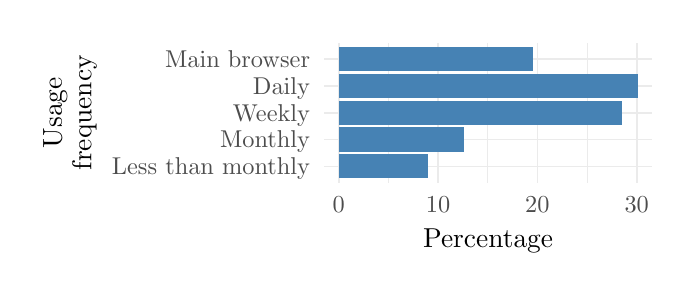
\begin{tikzpicture}[x=1pt,y=1pt]
\definecolor{fillColor}{RGB}{255,255,255}
\path[use as bounding box,fill=fillColor,fill opacity=0.00] (0,0) rectangle (231.26, 86.72);
\begin{scope}
\path[clip] (106.99, 30.77) rectangle (225.76, 81.22);
\definecolor{drawColor}{gray}{0.92}

\path[draw=drawColor,line width= 0.3pt,line join=round] (130.33, 30.77) --
	(130.33, 81.22);

\path[draw=drawColor,line width= 0.3pt,line join=round] (166.23, 30.77) --
	(166.23, 81.22);

\path[draw=drawColor,line width= 0.3pt,line join=round] (202.13, 30.77) --
	(202.13, 81.22);

\path[draw=drawColor,line width= 0.6pt,line join=round] (106.99, 36.59) --
	(225.76, 36.59);

\path[draw=drawColor,line width= 0.6pt,line join=round] (106.99, 46.30) --
	(225.76, 46.30);

\path[draw=drawColor,line width= 0.6pt,line join=round] (106.99, 56.00) --
	(225.76, 56.00);

\path[draw=drawColor,line width= 0.6pt,line join=round] (106.99, 65.70) --
	(225.76, 65.70);

\path[draw=drawColor,line width= 0.6pt,line join=round] (106.99, 75.40) --
	(225.76, 75.40);

\path[draw=drawColor,line width= 0.6pt,line join=round] (112.38, 30.77) --
	(112.38, 81.22);

\path[draw=drawColor,line width= 0.6pt,line join=round] (148.28, 30.77) --
	(148.28, 81.22);

\path[draw=drawColor,line width= 0.6pt,line join=round] (184.18, 30.77) --
	(184.18, 81.22);

\path[draw=drawColor,line width= 0.6pt,line join=round] (220.08, 30.77) --
	(220.08, 81.22);
\definecolor{fillColor}{RGB}{70,130,180}

\path[fill=fillColor] (112.38, 32.23) rectangle (144.69, 40.96);

\path[fill=fillColor] (112.38, 41.93) rectangle (157.76, 50.66);

\path[fill=fillColor] (112.38, 51.63) rectangle (214.84, 60.36);

\path[fill=fillColor] (112.38, 61.33) rectangle (220.36, 70.07);

\path[fill=fillColor] (112.38, 71.04) rectangle (182.53, 79.77);
\end{scope}
\begin{scope}
\path[clip] (  0.00,  0.00) rectangle (231.26, 86.72);
\definecolor{drawColor}{gray}{0.30}

\node[text=drawColor,anchor=base east,inner sep=0pt, outer sep=0pt, scale=  0.88] at (102.04, 33.56) {Less than monthly};

\node[text=drawColor,anchor=base east,inner sep=0pt, outer sep=0pt, scale=  0.88] at (102.04, 43.27) {Monthly};

\node[text=drawColor,anchor=base east,inner sep=0pt, outer sep=0pt, scale=  0.88] at (102.04, 52.97) {Weekly};

\node[text=drawColor,anchor=base east,inner sep=0pt, outer sep=0pt, scale=  0.88] at (102.04, 62.67) {Daily};

\node[text=drawColor,anchor=base east,inner sep=0pt, outer sep=0pt, scale=  0.88] at (102.04, 72.37) {Main browser};
\end{scope}
\begin{scope}
\path[clip] (  0.00,  0.00) rectangle (231.26, 86.72);
\definecolor{drawColor}{gray}{0.30}

\node[text=drawColor,anchor=base,inner sep=0pt, outer sep=0pt, scale=  0.88] at (112.38, 19.76) {0};

\node[text=drawColor,anchor=base,inner sep=0pt, outer sep=0pt, scale=  0.88] at (148.28, 19.76) {10};

\node[text=drawColor,anchor=base,inner sep=0pt, outer sep=0pt, scale=  0.88] at (184.18, 19.76) {20};

\node[text=drawColor,anchor=base,inner sep=0pt, outer sep=0pt, scale=  0.88] at (220.08, 19.76) {30};
\end{scope}
\begin{scope}
\path[clip] (  0.00,  0.00) rectangle (231.26, 86.72);
\definecolor{drawColor}{RGB}{0,0,0}

\node[text=drawColor,anchor=base,inner sep=0pt, outer sep=0pt, scale=  0.99] at (166.37,  7.44) {Percentage};
\end{scope}
\begin{scope}
\path[clip] (  0.00,  0.00) rectangle (231.26, 86.72);
\definecolor{drawColor}{RGB}{0,0,0}

\node[text=drawColor,rotate= 90.00,anchor=base,inner sep=0pt, outer sep=0pt, scale=  0.99] at ( 12.32, 56.00) {Usage};

\node[text=drawColor,rotate= 90.00,anchor=base,inner sep=0pt, outer sep=0pt, scale=  0.99] at ( 23.01, 56.00) {frequency};
\end{scope}
\end{tikzpicture}

    \caption{The usage frequency of Tor Browser among our respondents.  Almost
    half of our respondents use Tor Browser either daily or as their main
    browser.}
    \label{fig:tor-usage}
\end{figure}

\begin{figure}[t]
    \centering
    % Created by tikzDevice version 0.10.1 on 2018-02-09 14:33:04
% !TEX encoding = UTF-8 Unicode
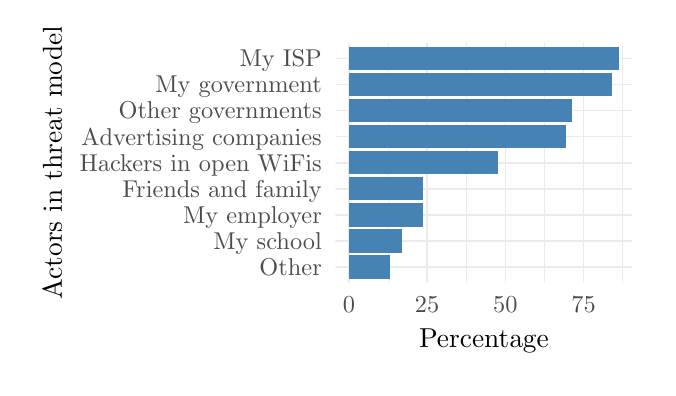
\begin{tikzpicture}[x=1pt,y=1pt]
\definecolor{fillColor}{RGB}{255,255,255}
\path[use as bounding box,fill=fillColor,fill opacity=0.00] (0,0) rectangle (224.04,122.86);
\begin{scope}
\path[clip] (111.23, 30.77) rectangle (218.54,117.36);
\definecolor{drawColor}{gray}{0.92}

\path[draw=drawColor,line width= 0.3pt,line join=round] (130.23, 30.77) --
	(130.23,117.36);

\path[draw=drawColor,line width= 0.3pt,line join=round] (158.48, 30.77) --
	(158.48,117.36);

\path[draw=drawColor,line width= 0.3pt,line join=round] (186.72, 30.77) --
	(186.72,117.36);

\path[draw=drawColor,line width= 0.3pt,line join=round] (214.97, 30.77) --
	(214.97,117.36);

\path[draw=drawColor,line width= 0.6pt,line join=round] (111.23, 36.42) --
	(218.54, 36.42);

\path[draw=drawColor,line width= 0.6pt,line join=round] (111.23, 45.83) --
	(218.54, 45.83);

\path[draw=drawColor,line width= 0.6pt,line join=round] (111.23, 55.24) --
	(218.54, 55.24);

\path[draw=drawColor,line width= 0.6pt,line join=round] (111.23, 64.65) --
	(218.54, 64.65);

\path[draw=drawColor,line width= 0.6pt,line join=round] (111.23, 74.07) --
	(218.54, 74.07);

\path[draw=drawColor,line width= 0.6pt,line join=round] (111.23, 83.48) --
	(218.54, 83.48);

\path[draw=drawColor,line width= 0.6pt,line join=round] (111.23, 92.89) --
	(218.54, 92.89);

\path[draw=drawColor,line width= 0.6pt,line join=round] (111.23,102.30) --
	(218.54,102.30);

\path[draw=drawColor,line width= 0.6pt,line join=round] (111.23,111.71) --
	(218.54,111.71);

\path[draw=drawColor,line width= 0.6pt,line join=round] (116.11, 30.77) --
	(116.11,117.36);

\path[draw=drawColor,line width= 0.6pt,line join=round] (144.35, 30.77) --
	(144.35,117.36);

\path[draw=drawColor,line width= 0.6pt,line join=round] (172.60, 30.77) --
	(172.60,117.36);

\path[draw=drawColor,line width= 0.6pt,line join=round] (200.85, 30.77) --
	(200.85,117.36);
\definecolor{fillColor}{RGB}{70,130,180}

\path[fill=fillColor] (116.11, 32.18) rectangle (130.90, 40.66);

\path[fill=fillColor] (116.11, 41.60) rectangle (135.19, 50.07);

\path[fill=fillColor] (116.11, 51.01) rectangle (142.69, 59.48);

\path[fill=fillColor] (116.11, 60.42) rectangle (142.91, 68.89);

\path[fill=fillColor] (116.11, 69.83) rectangle (169.92, 78.30);

\path[fill=fillColor] (116.11, 79.24) rectangle (194.36, 87.71);

\path[fill=fillColor] (116.11, 88.65) rectangle (196.72, 97.12);

\path[fill=fillColor] (116.11, 98.07) rectangle (211.30,106.54);

\path[fill=fillColor] (116.11,107.48) rectangle (213.66,115.95);
\end{scope}
\begin{scope}
\path[clip] (  0.00,  0.00) rectangle (224.04,122.86);
\definecolor{drawColor}{gray}{0.30}

\node[text=drawColor,anchor=base east,inner sep=0pt, outer sep=0pt, scale=  0.88] at (106.28, 33.39) {Other};

\node[text=drawColor,anchor=base east,inner sep=0pt, outer sep=0pt, scale=  0.88] at (106.28, 42.80) {My school};

\node[text=drawColor,anchor=base east,inner sep=0pt, outer sep=0pt, scale=  0.88] at (106.28, 52.21) {My employer};

\node[text=drawColor,anchor=base east,inner sep=0pt, outer sep=0pt, scale=  0.88] at (106.28, 61.62) {Friends and family};

\node[text=drawColor,anchor=base east,inner sep=0pt, outer sep=0pt, scale=  0.88] at (106.28, 71.04) {Hackers in open WiFis};

\node[text=drawColor,anchor=base east,inner sep=0pt, outer sep=0pt, scale=  0.88] at (106.28, 80.45) {Advertising companies};

\node[text=drawColor,anchor=base east,inner sep=0pt, outer sep=0pt, scale=  0.88] at (106.28, 89.86) {Other governments};

\node[text=drawColor,anchor=base east,inner sep=0pt, outer sep=0pt, scale=  0.88] at (106.28, 99.27) {My government};

\node[text=drawColor,anchor=base east,inner sep=0pt, outer sep=0pt, scale=  0.88] at (106.28,108.68) {My ISP};
\end{scope}
\begin{scope}
\path[clip] (  0.00,  0.00) rectangle (224.04,122.86);
\definecolor{drawColor}{gray}{0.30}

\node[text=drawColor,anchor=base,inner sep=0pt, outer sep=0pt, scale=  0.88] at (116.11, 19.76) {0};

\node[text=drawColor,anchor=base,inner sep=0pt, outer sep=0pt, scale=  0.88] at (144.35, 19.76) {25};

\node[text=drawColor,anchor=base,inner sep=0pt, outer sep=0pt, scale=  0.88] at (172.60, 19.76) {50};

\node[text=drawColor,anchor=base,inner sep=0pt, outer sep=0pt, scale=  0.88] at (200.85, 19.76) {75};
\end{scope}
\begin{scope}
\path[clip] (  0.00,  0.00) rectangle (224.04,122.86);
\definecolor{drawColor}{RGB}{0,0,0}

\node[text=drawColor,anchor=base,inner sep=0pt, outer sep=0pt, scale=  0.99] at (164.88,  7.44) {Percentage};
\end{scope}
\begin{scope}
\path[clip] (  0.00,  0.00) rectangle (224.04,122.86);
\definecolor{drawColor}{RGB}{0,0,0}

\node[text=drawColor,rotate= 90.00,anchor=base,inner sep=0pt, outer sep=0pt, scale=  0.99] at ( 12.32, 74.07) {Actors in threat model};
\end{scope}
\end{tikzpicture}

    \caption{The threat actors that our respondents seek to protect themselves
        from by using Tor Browser.}
    \label{fig:tor-threats}
\end{figure}

People who selected ``Other'' gave a variety of responses.  A number of
respondents specifically pointed out Google and Facebook.  ISPs, backbone ISPs,
and web sites were another common theme.  A number of respondents are struggling
with personal threats that include identity theft, targeted harassment, and
stalking.  Research is another common theme: Several respondents want to learn
about a topic without revealing their interest in it.  Some respondents use Tor
for search engine optimization, computer security research, and to research
medical conditions.  Finally, Tor provides technical advantages that don't
involve a threat actor.  Some respondents want IPv6 connectivity, evasion of
geographical content restrictions, and access to onion services.  A small number
of respondents are only interested in technical aspects other than privacy.  One
respondent stated that they don't need anonymity themselves but instead use Tor
to provide cover traffic for ``people who need protection.''

\subsubsection{Onion service usage}

The usage frequency of onion services is almost uniformly distributed among our
respondents; 24\% use onion sites less than once a month, 22\% use them about
monthly, 25\% weekly, and 23\% daily.  The remaining 6\% has never used an onion
service before.

The majority of our respondents (61.8\%) has used onion services for purposes
other than web browsing before.  Several protocols such as the chat application
Ricochet~\cite{ricochet} and the file sharing application
OnionShare~\cite{onionshare} were purpose-built on top of onion services while
existing TCP-based tools such as SSH can also be used with onion addresses
instead of traditional IP addresses.  Almost one third (29.7\%) of our
participants use onion service for non-browsing activities at least once a week.

But why do Tor users browse onion services in the first place?
Figure~\ref{fig:onion-usage} provides an answer.  The majority uses onion
services because of the additional anonymity (70\%) and the additional security
(61\%).  For 46\% it is the only way to access some content they enjoy, so using
onion services is a necessity.  27\% of our respondents found themselves curious
about the ``Dark Web'' and set out to find their own answer and 19\%
occasionally stumble upon links to onion services in their day-to-day browsing
activity.  Respondents who selected ``Other'' gave a variety of reasons, the
most predominant of which was the ability to set up a TCP service behind a NAT
device.  That way, it is possible to run an SSH server in a home network that
has neither a permanent IP address, nor port forwarding.  Other noteworthy
respondents use onion services to reduce the load on exit relays, to do
technical research, and to access sites that are otherwise unavailable.

\begin{figure}[t]
    \centering
    % Created by tikzDevice version 0.10.1 on 2018-01-12 16:14:57
% !TEX encoding = UTF-8 Unicode
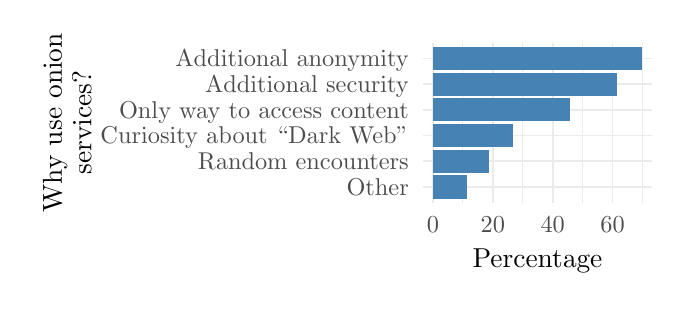
\begin{tikzpicture}[x=1pt,y=1pt]
\definecolor{fillColor}{RGB}{255,255,255}
\path[use as bounding box,fill=fillColor,fill opacity=0.00] (0,0) rectangle (231.26, 93.95);
\begin{scope}
\path[clip] (142.68, 30.77) rectangle (225.76, 88.45);
\definecolor{drawColor}{gray}{0.92}

\path[draw=drawColor,line width= 0.3pt,line join=round] (157.27, 30.77) --
	(157.27, 88.45);

\path[draw=drawColor,line width= 0.3pt,line join=round] (178.90, 30.77) --
	(178.90, 88.45);

\path[draw=drawColor,line width= 0.3pt,line join=round] (200.54, 30.77) --
	(200.54, 88.45);

\path[draw=drawColor,line width= 0.3pt,line join=round] (222.17, 30.77) --
	(222.17, 88.45);

\path[draw=drawColor,line width= 0.6pt,line join=round] (142.68, 36.35) --
	(225.76, 36.35);

\path[draw=drawColor,line width= 0.6pt,line join=round] (142.68, 45.66) --
	(225.76, 45.66);

\path[draw=drawColor,line width= 0.6pt,line join=round] (142.68, 54.96) --
	(225.76, 54.96);

\path[draw=drawColor,line width= 0.6pt,line join=round] (142.68, 64.26) --
	(225.76, 64.26);

\path[draw=drawColor,line width= 0.6pt,line join=round] (142.68, 73.57) --
	(225.76, 73.57);

\path[draw=drawColor,line width= 0.6pt,line join=round] (142.68, 82.87) --
	(225.76, 82.87);

\path[draw=drawColor,line width= 0.6pt,line join=round] (146.45, 30.77) --
	(146.45, 88.45);

\path[draw=drawColor,line width= 0.6pt,line join=round] (168.09, 30.77) --
	(168.09, 88.45);

\path[draw=drawColor,line width= 0.6pt,line join=round] (189.72, 30.77) --
	(189.72, 88.45);

\path[draw=drawColor,line width= 0.6pt,line join=round] (211.35, 30.77) --
	(211.35, 88.45);
\definecolor{fillColor}{RGB}{70,130,180}

\path[fill=fillColor] (146.45, 32.17) rectangle (158.77, 40.54);

\path[fill=fillColor] (146.45, 41.47) rectangle (166.57, 49.84);

\path[fill=fillColor] (146.45, 50.77) rectangle (175.40, 59.15);

\path[fill=fillColor] (146.45, 60.08) rectangle (196.12, 68.45);

\path[fill=fillColor] (146.45, 69.38) rectangle (212.96, 77.75);

\path[fill=fillColor] (146.45, 78.68) rectangle (221.99, 87.06);
\end{scope}
\begin{scope}
\path[clip] (  0.00,  0.00) rectangle (231.26, 93.95);
\definecolor{drawColor}{gray}{0.30}

\node[text=drawColor,anchor=base east,inner sep=0pt, outer sep=0pt, scale=  0.88] at (137.73, 33.32) {Other};

\node[text=drawColor,anchor=base east,inner sep=0pt, outer sep=0pt, scale=  0.88] at (137.73, 42.63) {Random encounters};

\node[text=drawColor,anchor=base east,inner sep=0pt, outer sep=0pt, scale=  0.88] at (137.73, 51.93) {Curiosity about ``Dark Web''};

\node[text=drawColor,anchor=base east,inner sep=0pt, outer sep=0pt, scale=  0.88] at (137.73, 61.23) {Only way to access content};

\node[text=drawColor,anchor=base east,inner sep=0pt, outer sep=0pt, scale=  0.88] at (137.73, 70.54) {Additional security};

\node[text=drawColor,anchor=base east,inner sep=0pt, outer sep=0pt, scale=  0.88] at (137.73, 79.84) {Additional anonymity};
\end{scope}
\begin{scope}
\path[clip] (  0.00,  0.00) rectangle (231.26, 93.95);
\definecolor{drawColor}{gray}{0.30}

\node[text=drawColor,anchor=base,inner sep=0pt, outer sep=0pt, scale=  0.88] at (146.45, 19.76) {0};

\node[text=drawColor,anchor=base,inner sep=0pt, outer sep=0pt, scale=  0.88] at (168.09, 19.76) {20};

\node[text=drawColor,anchor=base,inner sep=0pt, outer sep=0pt, scale=  0.88] at (189.72, 19.76) {40};

\node[text=drawColor,anchor=base,inner sep=0pt, outer sep=0pt, scale=  0.88] at (211.35, 19.76) {60};
\end{scope}
\begin{scope}
\path[clip] (  0.00,  0.00) rectangle (231.26, 93.95);
\definecolor{drawColor}{RGB}{0,0,0}

\node[text=drawColor,anchor=base,inner sep=0pt, outer sep=0pt, scale=  0.99] at (184.22,  7.44) {Percentage};
\end{scope}
\begin{scope}
\path[clip] (  0.00,  0.00) rectangle (231.26, 93.95);
\definecolor{drawColor}{RGB}{0,0,0}

\node[text=drawColor,rotate= 90.00,anchor=base,inner sep=0pt, outer sep=0pt, scale=  0.99] at ( 12.32, 59.61) {Why use onion};

\node[text=drawColor,rotate= 90.00,anchor=base,inner sep=0pt, outer sep=0pt, scale=  0.99] at ( 23.01, 59.61) {services?};
\end{scope}
\end{tikzpicture}

    \caption{Our respondents' (multiple choice) reasons for using onion
    services.}
    \label{fig:onion-usage}
\end{figure}

\subsubsection{Onion service discovery}

Recall that onion services are private by default, leaving it up to their
operator to disseminate the domain.  Established search engines such as Google
are therefore inadequate to find content on onion services.  We wanted to find
out how our respondents discover onion services.
Figure~\ref{fig:onion-discovery} illustrates the results.  The three most
popular ways of discovering new onion sites, all approximating 50\%, are social
networking sites such as Twitter and Reddit, the list of search engines such as
Ahmia\footnote{Ahmia.fi is an onion site search engine that crawls
user-submitted onion domains.  It publishes the list of all indexed onion
services at \url{https://ahmia.fi/onions/}.}, and randomly encountering links
when browsing the web.

While significantly less popular, discovering onion domains through friends and
family has the advantage of trust.  Some of our interview participant indicated
that they heavily rely on this distribution method simply because they can trust
the origin.  Finally, a mere 4\% indicated that they are not interested in
learning about new onion services.

Respondents who selected ``Other'' predominantly brought up
independently-maintained lists of onion services and aggregators.  A noteworthy
example is the Hidden Wiki.

\begin{figure}[t]
    \centering
    % Created by tikzDevice version 0.10.1 on 2018-01-12 16:15:03
% !TEX encoding = UTF-8 Unicode
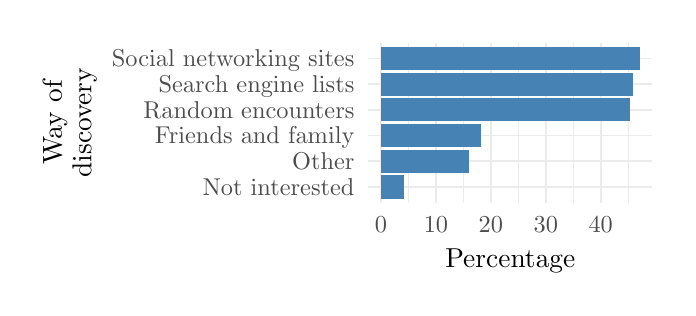
\begin{tikzpicture}[x=1pt,y=1pt]
\definecolor{fillColor}{RGB}{255,255,255}
\path[use as bounding box,fill=fillColor,fill opacity=0.00] (0,0) rectangle (231.26, 93.95);
\begin{scope}
\path[clip] (123.02, 30.77) rectangle (225.76, 88.45);
\definecolor{drawColor}{gray}{0.92}

\path[draw=drawColor,line width= 0.3pt,line join=round] (137.61, 30.77) --
	(137.61, 88.45);

\path[draw=drawColor,line width= 0.3pt,line join=round] (157.46, 30.77) --
	(157.46, 88.45);

\path[draw=drawColor,line width= 0.3pt,line join=round] (177.31, 30.77) --
	(177.31, 88.45);

\path[draw=drawColor,line width= 0.3pt,line join=round] (197.16, 30.77) --
	(197.16, 88.45);

\path[draw=drawColor,line width= 0.3pt,line join=round] (217.00, 30.77) --
	(217.00, 88.45);

\path[draw=drawColor,line width= 0.6pt,line join=round] (123.02, 36.35) --
	(225.76, 36.35);

\path[draw=drawColor,line width= 0.6pt,line join=round] (123.02, 45.66) --
	(225.76, 45.66);

\path[draw=drawColor,line width= 0.6pt,line join=round] (123.02, 54.96) --
	(225.76, 54.96);

\path[draw=drawColor,line width= 0.6pt,line join=round] (123.02, 64.26) --
	(225.76, 64.26);

\path[draw=drawColor,line width= 0.6pt,line join=round] (123.02, 73.57) --
	(225.76, 73.57);

\path[draw=drawColor,line width= 0.6pt,line join=round] (123.02, 82.87) --
	(225.76, 82.87);

\path[draw=drawColor,line width= 0.6pt,line join=round] (127.69, 30.77) --
	(127.69, 88.45);

\path[draw=drawColor,line width= 0.6pt,line join=round] (147.54, 30.77) --
	(147.54, 88.45);

\path[draw=drawColor,line width= 0.6pt,line join=round] (167.38, 30.77) --
	(167.38, 88.45);

\path[draw=drawColor,line width= 0.6pt,line join=round] (187.23, 30.77) --
	(187.23, 88.45);

\path[draw=drawColor,line width= 0.6pt,line join=round] (207.08, 30.77) --
	(207.08, 88.45);
\definecolor{fillColor}{RGB}{70,130,180}

\path[fill=fillColor] (127.69, 32.17) rectangle (135.96, 40.54);

\path[fill=fillColor] (127.69, 41.47) rectangle (159.33, 49.84);

\path[fill=fillColor] (127.69, 50.77) rectangle (163.85, 59.15);

\path[fill=fillColor] (127.69, 60.08) rectangle (217.70, 68.45);

\path[fill=fillColor] (127.69, 69.38) rectangle (218.83, 77.75);

\path[fill=fillColor] (127.69, 78.68) rectangle (221.09, 87.06);
\end{scope}
\begin{scope}
\path[clip] (  0.00,  0.00) rectangle (231.26, 93.95);
\definecolor{drawColor}{gray}{0.30}

\node[text=drawColor,anchor=base east,inner sep=0pt, outer sep=0pt, scale=  0.88] at (118.07, 33.32) {Not interested};

\node[text=drawColor,anchor=base east,inner sep=0pt, outer sep=0pt, scale=  0.88] at (118.07, 42.63) {Other};

\node[text=drawColor,anchor=base east,inner sep=0pt, outer sep=0pt, scale=  0.88] at (118.07, 51.93) {Friends and family};

\node[text=drawColor,anchor=base east,inner sep=0pt, outer sep=0pt, scale=  0.88] at (118.07, 61.23) {Random encounters};

\node[text=drawColor,anchor=base east,inner sep=0pt, outer sep=0pt, scale=  0.88] at (118.07, 70.54) {Search engine lists};

\node[text=drawColor,anchor=base east,inner sep=0pt, outer sep=0pt, scale=  0.88] at (118.07, 79.84) {Social networking sites};
\end{scope}
\begin{scope}
\path[clip] (  0.00,  0.00) rectangle (231.26, 93.95);
\definecolor{drawColor}{gray}{0.30}

\node[text=drawColor,anchor=base,inner sep=0pt, outer sep=0pt, scale=  0.88] at (127.69, 19.76) {0};

\node[text=drawColor,anchor=base,inner sep=0pt, outer sep=0pt, scale=  0.88] at (147.54, 19.76) {10};

\node[text=drawColor,anchor=base,inner sep=0pt, outer sep=0pt, scale=  0.88] at (167.38, 19.76) {20};

\node[text=drawColor,anchor=base,inner sep=0pt, outer sep=0pt, scale=  0.88] at (187.23, 19.76) {30};

\node[text=drawColor,anchor=base,inner sep=0pt, outer sep=0pt, scale=  0.88] at (207.08, 19.76) {40};
\end{scope}
\begin{scope}
\path[clip] (  0.00,  0.00) rectangle (231.26, 93.95);
\definecolor{drawColor}{RGB}{0,0,0}

\node[text=drawColor,anchor=base,inner sep=0pt, outer sep=0pt, scale=  0.99] at (174.39,  7.44) {Percentage};
\end{scope}
\begin{scope}
\path[clip] (  0.00,  0.00) rectangle (231.26, 93.95);
\definecolor{drawColor}{RGB}{0,0,0}

\node[text=drawColor,rotate= 90.00,anchor=base,inner sep=0pt, outer sep=0pt, scale=  0.99] at ( 12.32, 59.61) {Way of};

\node[text=drawColor,rotate= 90.00,anchor=base,inner sep=0pt, outer sep=0pt, scale=  0.99] at ( 23.01, 59.61) {discovery};
\end{scope}
\end{tikzpicture}

    \caption{Our respondents' (multiple choice) methods of discovering onion
    services.}
    \label{fig:onion-discovery}
\end{figure}

The next question in our survey then asked if our respondents are satisfied with
the way they discover onion services.  60\% selected ``Yes'' while 40\% selected
``No.'' Some respondents who selected ``Yes'' brought up that they have no
interest in learning about new onion services, in part because they only use a
small set of onion services.  Among the people who are not satisfied, the most
prominent complaint was about broken links on onion site lists.  There is
non-trivial churn among onion sites and our respondents were frustrated that
existing lists are typically not curated and contain many dead links.

Many respondents were not aware of search engines such as ahmia.fi.  Among those
that were, many were not satisfied with both the search results and the number
of indexed onion sites.  Unsurprisingly, a ``Google for onion sites'' was a
frequent wish.

Several respondents were unhappy with existing aggregators.  In addition to
broken links, some distrust lists because they occasionally contain scam and
phishing sites.  The difficulty of telling apart two given onion domain names
exacerbates this issue.  Another common wish for aggregators was for them to be
more verbose in their description of onion sites.  In particular, some
respondents want to avoid illegal and pornographic content, which is often
difficult if the description is vague and the onion domain reveals nothing about
its content.

Many respondents expressed frustration about the difficulty of finding out if
site X also provides a corresponding onion service.  A common wish was to have
site X list its onion service prominently in a footer.  Ironically, some
respondents were surprised that torproject.org has a corresponding onion site --
they couldn't find it on the web site.

Interestingly, some respondents voiced frustration about various usability
issues, but mentioned in the same sentence that this is an inherent trade-off of
privacy technology, suggesting that there is nothing that can be done about it.

\subsubsection{Onion service domain format}

Conventional domains are designed to be easy to remember and recognize.  But how do users
handle the randomly-generated onion domains?  Question 3.8 in our survey asked
exactly that, with the responses being illustrated in
Figure~\ref{fig:onion-domain-mgmt}.

\begin{figure}[t]
    \centering
    % Created by tikzDevice version 0.10.1 on 2018-02-09 14:36:33
% !TEX encoding = UTF-8 Unicode
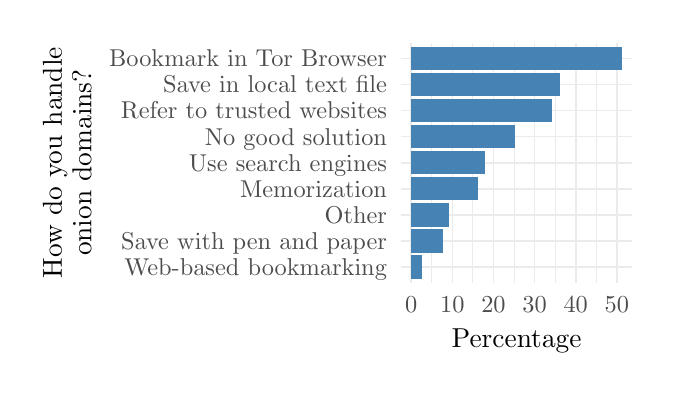
\begin{tikzpicture}[x=1pt,y=1pt]
\definecolor{fillColor}{RGB}{255,255,255}
\path[use as bounding box,fill=fillColor,fill opacity=0.00] (0,0) rectangle (224.04,122.86);
\begin{scope}
\path[clip] (134.78, 30.77) rectangle (218.54,117.36);
\definecolor{drawColor}{gray}{0.92}

\path[draw=drawColor,line width= 0.3pt,line join=round] (146.02, 30.77) --
	(146.02,117.36);

\path[draw=drawColor,line width= 0.3pt,line join=round] (160.88, 30.77) --
	(160.88,117.36);

\path[draw=drawColor,line width= 0.3pt,line join=round] (175.74, 30.77) --
	(175.74,117.36);

\path[draw=drawColor,line width= 0.3pt,line join=round] (190.61, 30.77) --
	(190.61,117.36);

\path[draw=drawColor,line width= 0.3pt,line join=round] (205.47, 30.77) --
	(205.47,117.36);

\path[draw=drawColor,line width= 0.6pt,line join=round] (134.78, 36.42) --
	(218.54, 36.42);

\path[draw=drawColor,line width= 0.6pt,line join=round] (134.78, 45.83) --
	(218.54, 45.83);

\path[draw=drawColor,line width= 0.6pt,line join=round] (134.78, 55.24) --
	(218.54, 55.24);

\path[draw=drawColor,line width= 0.6pt,line join=round] (134.78, 64.65) --
	(218.54, 64.65);

\path[draw=drawColor,line width= 0.6pt,line join=round] (134.78, 74.07) --
	(218.54, 74.07);

\path[draw=drawColor,line width= 0.6pt,line join=round] (134.78, 83.48) --
	(218.54, 83.48);

\path[draw=drawColor,line width= 0.6pt,line join=round] (134.78, 92.89) --
	(218.54, 92.89);

\path[draw=drawColor,line width= 0.6pt,line join=round] (134.78,102.30) --
	(218.54,102.30);

\path[draw=drawColor,line width= 0.6pt,line join=round] (134.78,111.71) --
	(218.54,111.71);

\path[draw=drawColor,line width= 0.6pt,line join=round] (138.58, 30.77) --
	(138.58,117.36);

\path[draw=drawColor,line width= 0.6pt,line join=round] (153.45, 30.77) --
	(153.45,117.36);

\path[draw=drawColor,line width= 0.6pt,line join=round] (168.31, 30.77) --
	(168.31,117.36);

\path[draw=drawColor,line width= 0.6pt,line join=round] (183.17, 30.77) --
	(183.17,117.36);

\path[draw=drawColor,line width= 0.6pt,line join=round] (198.04, 30.77) --
	(198.04,117.36);

\path[draw=drawColor,line width= 0.6pt,line join=round] (212.90, 30.77) --
	(212.90,117.36);
\definecolor{fillColor}{RGB}{70,130,180}

\path[fill=fillColor] (138.58, 32.18) rectangle (142.54, 40.66);

\path[fill=fillColor] (138.58, 41.60) rectangle (150.15, 50.07);

\path[fill=fillColor] (138.58, 51.01) rectangle (152.13, 59.48);

\path[fill=fillColor] (138.58, 60.42) rectangle (162.84, 68.89);

\path[fill=fillColor] (138.58, 69.83) rectangle (165.10, 78.30);

\path[fill=fillColor] (138.58, 79.24) rectangle (176.10, 87.71);

\path[fill=fillColor] (138.58, 88.65) rectangle (189.36, 97.12);

\path[fill=fillColor] (138.58, 98.07) rectangle (192.45,106.54);

\path[fill=fillColor] (138.58,107.48) rectangle (214.73,115.95);
\end{scope}
\begin{scope}
\path[clip] (  0.00,  0.00) rectangle (224.04,122.86);
\definecolor{drawColor}{gray}{0.30}

\node[text=drawColor,anchor=base east,inner sep=0pt, outer sep=0pt, scale=  0.88] at (129.83, 33.39) {Web-based bookmarking};

\node[text=drawColor,anchor=base east,inner sep=0pt, outer sep=0pt, scale=  0.88] at (129.83, 42.80) {Save with pen and paper};

\node[text=drawColor,anchor=base east,inner sep=0pt, outer sep=0pt, scale=  0.88] at (129.83, 52.21) {Other};

\node[text=drawColor,anchor=base east,inner sep=0pt, outer sep=0pt, scale=  0.88] at (129.83, 61.62) {Memorization};

\node[text=drawColor,anchor=base east,inner sep=0pt, outer sep=0pt, scale=  0.88] at (129.83, 71.04) {Use search engines};

\node[text=drawColor,anchor=base east,inner sep=0pt, outer sep=0pt, scale=  0.88] at (129.83, 80.45) {No good solution};

\node[text=drawColor,anchor=base east,inner sep=0pt, outer sep=0pt, scale=  0.88] at (129.83, 89.86) {Refer to trusted websites};

\node[text=drawColor,anchor=base east,inner sep=0pt, outer sep=0pt, scale=  0.88] at (129.83, 99.27) {Save in local text file};

\node[text=drawColor,anchor=base east,inner sep=0pt, outer sep=0pt, scale=  0.88] at (129.83,108.68) {Bookmark in Tor Browser};
\end{scope}
\begin{scope}
\path[clip] (  0.00,  0.00) rectangle (224.04,122.86);
\definecolor{drawColor}{gray}{0.30}

\node[text=drawColor,anchor=base,inner sep=0pt, outer sep=0pt, scale=  0.88] at (138.58, 19.76) {0};

\node[text=drawColor,anchor=base,inner sep=0pt, outer sep=0pt, scale=  0.88] at (153.45, 19.76) {10};

\node[text=drawColor,anchor=base,inner sep=0pt, outer sep=0pt, scale=  0.88] at (168.31, 19.76) {20};

\node[text=drawColor,anchor=base,inner sep=0pt, outer sep=0pt, scale=  0.88] at (183.17, 19.76) {30};

\node[text=drawColor,anchor=base,inner sep=0pt, outer sep=0pt, scale=  0.88] at (198.04, 19.76) {40};

\node[text=drawColor,anchor=base,inner sep=0pt, outer sep=0pt, scale=  0.88] at (212.90, 19.76) {50};
\end{scope}
\begin{scope}
\path[clip] (  0.00,  0.00) rectangle (224.04,122.86);
\definecolor{drawColor}{RGB}{0,0,0}

\node[text=drawColor,anchor=base,inner sep=0pt, outer sep=0pt, scale=  0.99] at (176.66,  7.44) {Percentage};
\end{scope}
\begin{scope}
\path[clip] (  0.00,  0.00) rectangle (224.04,122.86);
\definecolor{drawColor}{RGB}{0,0,0}

\node[text=drawColor,rotate= 90.00,anchor=base,inner sep=0pt, outer sep=0pt, scale=  0.99] at ( 12.32, 74.07) {How do you handle};

\node[text=drawColor,rotate= 90.00,anchor=base,inner sep=0pt, outer sep=0pt, scale=  0.99] at ( 23.01, 74.07) {onion domains?};
\end{scope}
\end{tikzpicture}

    \caption{The strategies that our respondents use to handle onion domains.
    More than half use bookmarks inside of Tor Browser and a quarter thinks that
    there's no good solution.}
    \label{fig:onion-domain-mgmt}
\end{figure}

Most respondents use bookmarks inside Tor Browser for onion domains.  While
convenient, it leaves a trace of (presumably) visited sites on one's computer.
One of Tor Browser's security requirements is ``disk avoidance,'' \ie, the
browser must not write anything to disk that would reveal the user's browsing
history~\cite[\S~2.1]{Perry2017a}.  Bookmarking links is a violation of this
security requirement.  Many of our respondents were aware of this issue.  About
a dozen respondents who selected ``Other'' stated that they store onion domains
encryptedly---either in a text file or in their password manager.

Somewhat less popular is saving onion domains in local text files (36\%),
getting them from trusted web sites (34\%), use search engines (18\%), memorize
domains (16\%), use some other techniques (9\%) or employ pen and paper (8\%).
Notably, one quarter of our respondents does not have a good solution to the
problem.  Given the alarming number of (possibly insecure) home-baked solutions,
a Tor Browser extension may be warranted to approach the problem.

The next question in our survey asked if our respondents expect the
next-generation domain format to change their browsing habits.  Interestingly,
only 17\% expect to have their browsing habits changed while 83\% don't.  Among
the respondents who selected ``Yes,'' many expressed that they memorize a small
number of onion domains (such as Facebook's), which will no longer be possible.
People who selected ``No'' mostly bring up that they treat onion domains as
opaque identifiers that they handle via tools such as bookmarks.  These results
suggest that the current state is dire, yet not expected to get much worse with
the new domain format.

Problematic:
``I only memorize the first part of the domain''

``If there isn't some cognizable word at the start, it'll be more difficult for
me to determine if I'm going to the correct domain or a scam. I may end up going
to less .onion sites as a result.''

\subsubsection{Onion service operation}

A survey question block on onion service operation shed light on the reasons for
running onion services and what sort of issues users face when doing so.  40\%
of our respondents once set up an onion service.  Among the respondents who
never have, 31\% have considered doing so while 30\% have never even considered
it.  Interestingly, 79\% of operators have run an onion service for private use
while 53\% have run them for the public.

Figure~\ref{fig:onion-operation-reasons} gives an overview of the reasons for
running onion services.  Interestingly, the extra security properties overshadow
the anonymity properties of onion services.  Another particularly popular reason
is NAT traversal---many respondents noted that onion services allow them to
expose a TCP service in their home network despite being behind a NAT device.
Finally, some people run onion service indirectly because third-party tools such
as OnionShare~\cite{onionshare} or Ricochet~\cite{ricochet} are built on top of
them.  Onion services can have clear benefits for businesses as well as
evidenced by one respondent who wrote on onion services: ``We use it for
delivering updates to our router to customers securely and without leaking
metadata.''

\begin{figure}[t]
    \centering
    % Created by tikzDevice version 0.10.1 on 2018-01-12 16:24:46
% !TEX encoding = UTF-8 Unicode
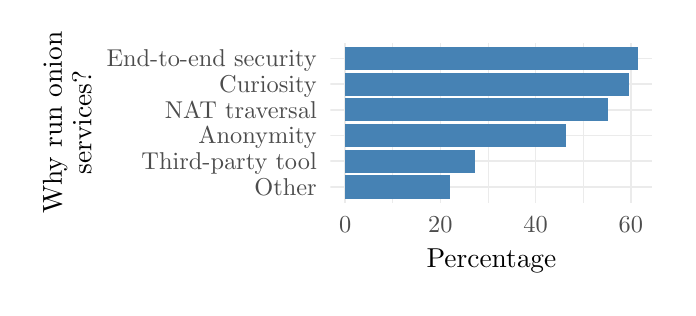
\begin{tikzpicture}[x=1pt,y=1pt]
\definecolor{fillColor}{RGB}{255,255,255}
\path[use as bounding box,fill=fillColor,fill opacity=0.00] (0,0) rectangle (231.26, 93.95);
\begin{scope}
\path[clip] (109.42, 30.77) rectangle (225.76, 88.45);
\definecolor{drawColor}{gray}{0.92}

\path[draw=drawColor,line width= 0.3pt,line join=round] (131.91, 30.77) --
	(131.91, 88.45);

\path[draw=drawColor,line width= 0.3pt,line join=round] (166.33, 30.77) --
	(166.33, 88.45);

\path[draw=drawColor,line width= 0.3pt,line join=round] (200.75, 30.77) --
	(200.75, 88.45);

\path[draw=drawColor,line width= 0.6pt,line join=round] (109.42, 36.35) --
	(225.76, 36.35);

\path[draw=drawColor,line width= 0.6pt,line join=round] (109.42, 45.66) --
	(225.76, 45.66);

\path[draw=drawColor,line width= 0.6pt,line join=round] (109.42, 54.96) --
	(225.76, 54.96);

\path[draw=drawColor,line width= 0.6pt,line join=round] (109.42, 64.26) --
	(225.76, 64.26);

\path[draw=drawColor,line width= 0.6pt,line join=round] (109.42, 73.57) --
	(225.76, 73.57);

\path[draw=drawColor,line width= 0.6pt,line join=round] (109.42, 82.87) --
	(225.76, 82.87);

\path[draw=drawColor,line width= 0.6pt,line join=round] (114.70, 30.77) --
	(114.70, 88.45);

\path[draw=drawColor,line width= 0.6pt,line join=round] (149.12, 30.77) --
	(149.12, 88.45);

\path[draw=drawColor,line width= 0.6pt,line join=round] (183.54, 30.77) --
	(183.54, 88.45);

\path[draw=drawColor,line width= 0.6pt,line join=round] (217.96, 30.77) --
	(217.96, 88.45);
\definecolor{fillColor}{RGB}{70,130,180}

\path[fill=fillColor] (114.70, 32.17) rectangle (152.48, 40.54);

\path[fill=fillColor] (114.70, 41.47) rectangle (161.72, 49.84);

\path[fill=fillColor] (114.70, 50.77) rectangle (194.45, 59.15);

\path[fill=fillColor] (114.70, 60.08) rectangle (209.56, 68.45);

\path[fill=fillColor] (114.70, 69.38) rectangle (217.12, 77.75);

\path[fill=fillColor] (114.70, 78.68) rectangle (220.48, 87.06);
\end{scope}
\begin{scope}
\path[clip] (  0.00,  0.00) rectangle (231.26, 93.95);
\definecolor{drawColor}{gray}{0.30}

\node[text=drawColor,anchor=base east,inner sep=0pt, outer sep=0pt, scale=  0.88] at (104.47, 33.32) {Other};

\node[text=drawColor,anchor=base east,inner sep=0pt, outer sep=0pt, scale=  0.88] at (104.47, 42.63) {Third-party tool};

\node[text=drawColor,anchor=base east,inner sep=0pt, outer sep=0pt, scale=  0.88] at (104.47, 51.93) {Anonymity};

\node[text=drawColor,anchor=base east,inner sep=0pt, outer sep=0pt, scale=  0.88] at (104.47, 61.23) {NAT traversal};

\node[text=drawColor,anchor=base east,inner sep=0pt, outer sep=0pt, scale=  0.88] at (104.47, 70.54) {Curiosity};

\node[text=drawColor,anchor=base east,inner sep=0pt, outer sep=0pt, scale=  0.88] at (104.47, 79.84) {End-to-end security};
\end{scope}
\begin{scope}
\path[clip] (  0.00,  0.00) rectangle (231.26, 93.95);
\definecolor{drawColor}{gray}{0.30}

\node[text=drawColor,anchor=base,inner sep=0pt, outer sep=0pt, scale=  0.88] at (114.70, 19.76) {0};

\node[text=drawColor,anchor=base,inner sep=0pt, outer sep=0pt, scale=  0.88] at (149.12, 19.76) {20};

\node[text=drawColor,anchor=base,inner sep=0pt, outer sep=0pt, scale=  0.88] at (183.54, 19.76) {40};

\node[text=drawColor,anchor=base,inner sep=0pt, outer sep=0pt, scale=  0.88] at (217.96, 19.76) {60};
\end{scope}
\begin{scope}
\path[clip] (  0.00,  0.00) rectangle (231.26, 93.95);
\definecolor{drawColor}{RGB}{0,0,0}

\node[text=drawColor,anchor=base,inner sep=0pt, outer sep=0pt, scale=  0.99] at (167.59,  7.44) {Percentage};
\end{scope}
\begin{scope}
\path[clip] (  0.00,  0.00) rectangle (231.26, 93.95);
\definecolor{drawColor}{RGB}{0,0,0}

\node[text=drawColor,rotate= 90.00,anchor=base,inner sep=0pt, outer sep=0pt, scale=  0.99] at ( 12.32, 59.61) {Why run onion};

\node[text=drawColor,rotate= 90.00,anchor=base,inner sep=0pt, outer sep=0pt, scale=  0.99] at ( 23.01, 59.61) {services?};
\end{scope}
\end{tikzpicture}

    \caption{The reasons people have for running onion services.}
    \label{fig:onion-operation-reasons}
\end{figure}

Figure~\ref{fig:onion-operation-concerns} illustrates the concerns that onion
service operators face.  We consider three attacks; \first somebody setting up a
phishing site for the operator's site, \second a denial-of-service attack, and
\third a deanonymization attack.  More than half of our respondents are at least
somewhat concerned about all of these attacks.  Almost 40\% claim to be
extremely concerned about somebody deanonymizing their onion service.  Indeed,
many respondents lamented the difficulty of knowing that an onion service setup
is robust against application-layer deanonymization attacks.

\begin{figure}[t]
    \centering
    % Created by tikzDevice version 0.10.1 on 2018-02-09 14:59:34
% !TEX encoding = UTF-8 Unicode
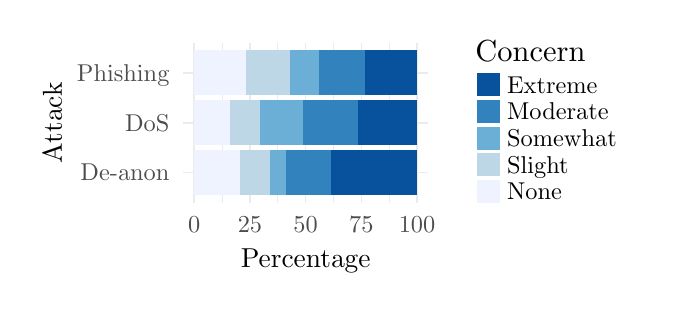
\begin{tikzpicture}[x=1pt,y=1pt]
\definecolor{fillColor}{RGB}{255,255,255}
\path[use as bounding box,fill=fillColor,fill opacity=0.00] (0,0) rectangle (224.04, 93.95);
\begin{scope}
\path[clip] ( 56.18, 30.77) rectangle (144.74, 88.45);
\definecolor{drawColor}{gray}{0.92}

\path[draw=drawColor,line width= 0.3pt,line join=round] ( 70.26, 30.77) --
	( 70.26, 88.45);

\path[draw=drawColor,line width= 0.3pt,line join=round] ( 90.39, 30.77) --
	( 90.39, 88.45);

\path[draw=drawColor,line width= 0.3pt,line join=round] (110.52, 30.77) --
	(110.52, 88.45);

\path[draw=drawColor,line width= 0.3pt,line join=round] (130.64, 30.77) --
	(130.64, 88.45);

\path[draw=drawColor,line width= 0.6pt,line join=round] ( 56.18, 41.59) --
	(144.74, 41.59);

\path[draw=drawColor,line width= 0.6pt,line join=round] ( 56.18, 59.61) --
	(144.74, 59.61);

\path[draw=drawColor,line width= 0.6pt,line join=round] ( 56.18, 77.64) --
	(144.74, 77.64);

\path[draw=drawColor,line width= 0.6pt,line join=round] ( 60.20, 30.77) --
	( 60.20, 88.45);

\path[draw=drawColor,line width= 0.6pt,line join=round] ( 80.33, 30.77) --
	( 80.33, 88.45);

\path[draw=drawColor,line width= 0.6pt,line join=round] (100.45, 30.77) --
	(100.45, 88.45);

\path[draw=drawColor,line width= 0.6pt,line join=round] (120.58, 30.77) --
	(120.58, 88.45);

\path[draw=drawColor,line width= 0.6pt,line join=round] (140.71, 30.77) --
	(140.71, 88.45);
\definecolor{fillColor}{RGB}{239,243,255}

\path[fill=fillColor] ( 60.20, 33.48) rectangle ( 76.78, 49.70);
\definecolor{fillColor}{RGB}{189,215,231}

\path[fill=fillColor] ( 76.78, 33.48) rectangle ( 87.44, 49.70);
\definecolor{fillColor}{RGB}{107,174,214}

\path[fill=fillColor] ( 87.44, 33.48) rectangle ( 93.35, 49.70);
\definecolor{fillColor}{RGB}{49,130,189}

\path[fill=fillColor] ( 93.35, 33.48) rectangle (109.54, 49.70);
\definecolor{fillColor}{RGB}{8,81,156}

\path[fill=fillColor] (109.54, 33.48) rectangle (140.72, 49.70);
\definecolor{fillColor}{RGB}{239,243,255}

\path[fill=fillColor] ( 60.20, 51.50) rectangle ( 73.16, 67.72);
\definecolor{fillColor}{RGB}{189,215,231}

\path[fill=fillColor] ( 73.16, 51.50) rectangle ( 83.77, 67.72);
\definecolor{fillColor}{RGB}{107,174,214}

\path[fill=fillColor] ( 83.77, 51.50) rectangle ( 99.47, 67.72);
\definecolor{fillColor}{RGB}{49,130,189}

\path[fill=fillColor] ( 99.47, 51.50) rectangle (119.50, 67.72);
\definecolor{fillColor}{RGB}{8,81,156}

\path[fill=fillColor] (119.50, 51.50) rectangle (140.71, 67.72);
\definecolor{fillColor}{RGB}{239,243,255}

\path[fill=fillColor] ( 60.20, 69.53) rectangle ( 79.05, 85.75);
\definecolor{fillColor}{RGB}{189,215,231}

\path[fill=fillColor] ( 79.05, 69.53) rectangle ( 94.75, 85.75);
\definecolor{fillColor}{RGB}{107,174,214}

\path[fill=fillColor] ( 94.75, 69.53) rectangle (105.36, 85.75);
\definecolor{fillColor}{RGB}{49,130,189}

\path[fill=fillColor] (105.36, 69.53) rectangle (121.85, 85.75);
\definecolor{fillColor}{RGB}{8,81,156}

\path[fill=fillColor] (121.85, 69.53) rectangle (140.70, 85.75);
\end{scope}
\begin{scope}
\path[clip] (  0.00,  0.00) rectangle (224.04, 93.95);
\definecolor{drawColor}{gray}{0.30}

\node[text=drawColor,anchor=base east,inner sep=0pt, outer sep=0pt, scale=  0.88] at ( 51.23, 38.56) {De-anon};

\node[text=drawColor,anchor=base east,inner sep=0pt, outer sep=0pt, scale=  0.88] at ( 51.23, 56.58) {DoS};

\node[text=drawColor,anchor=base east,inner sep=0pt, outer sep=0pt, scale=  0.88] at ( 51.23, 74.61) {Phishing};
\end{scope}
\begin{scope}
\path[clip] (  0.00,  0.00) rectangle (224.04, 93.95);
\definecolor{drawColor}{gray}{0.30}

\node[text=drawColor,anchor=base,inner sep=0pt, outer sep=0pt, scale=  0.88] at ( 60.20, 19.76) {0};

\node[text=drawColor,anchor=base,inner sep=0pt, outer sep=0pt, scale=  0.88] at ( 80.33, 19.76) {25};

\node[text=drawColor,anchor=base,inner sep=0pt, outer sep=0pt, scale=  0.88] at (100.45, 19.76) {50};

\node[text=drawColor,anchor=base,inner sep=0pt, outer sep=0pt, scale=  0.88] at (120.58, 19.76) {75};

\node[text=drawColor,anchor=base,inner sep=0pt, outer sep=0pt, scale=  0.88] at (140.71, 19.76) {100};
\end{scope}
\begin{scope}
\path[clip] (  0.00,  0.00) rectangle (224.04, 93.95);
\definecolor{drawColor}{RGB}{0,0,0}

\node[text=drawColor,anchor=base,inner sep=0pt, outer sep=0pt, scale=  0.99] at (100.46,  7.44) {Percentage};
\end{scope}
\begin{scope}
\path[clip] (  0.00,  0.00) rectangle (224.04, 93.95);
\definecolor{drawColor}{RGB}{0,0,0}

\node[text=drawColor,rotate= 90.00,anchor=base,inner sep=0pt, outer sep=0pt, scale=  0.99] at ( 12.32, 59.61) {Attack};
\end{scope}
\begin{scope}
\path[clip] (  0.00,  0.00) rectangle (224.04, 93.95);
\definecolor{drawColor}{RGB}{0,0,0}

\node[text=drawColor,anchor=base west,inner sep=0pt, outer sep=0pt, scale=  1.10] at (161.81, 81.72) {Concern};
\end{scope}
\begin{scope}
\path[clip] (  0.00,  0.00) rectangle (224.04, 93.95);
\definecolor{fillColor}{RGB}{8,81,156}

\path[fill=fillColor] (162.52, 69.18) rectangle (170.74, 77.40);
\end{scope}
\begin{scope}
\path[clip] (  0.00,  0.00) rectangle (224.04, 93.95);
\definecolor{fillColor}{RGB}{49,130,189}

\path[fill=fillColor] (162.52, 59.55) rectangle (170.74, 67.76);
\end{scope}
\begin{scope}
\path[clip] (  0.00,  0.00) rectangle (224.04, 93.95);
\definecolor{fillColor}{RGB}{107,174,214}

\path[fill=fillColor] (162.52, 49.91) rectangle (170.74, 58.12);
\end{scope}
\begin{scope}
\path[clip] (  0.00,  0.00) rectangle (224.04, 93.95);
\definecolor{fillColor}{RGB}{189,215,231}

\path[fill=fillColor] (162.52, 40.27) rectangle (170.74, 48.49);
\end{scope}
\begin{scope}
\path[clip] (  0.00,  0.00) rectangle (224.04, 93.95);
\definecolor{fillColor}{RGB}{239,243,255}

\path[fill=fillColor] (162.52, 30.64) rectangle (170.74, 38.85);
\end{scope}
\begin{scope}
\path[clip] (  0.00,  0.00) rectangle (224.04, 93.95);
\definecolor{drawColor}{RGB}{0,0,0}

\node[text=drawColor,anchor=base west,inner sep=0pt, outer sep=0pt, scale=  0.88] at (173.26, 70.26) {Extreme};
\end{scope}
\begin{scope}
\path[clip] (  0.00,  0.00) rectangle (224.04, 93.95);
\definecolor{drawColor}{RGB}{0,0,0}

\node[text=drawColor,anchor=base west,inner sep=0pt, outer sep=0pt, scale=  0.88] at (173.26, 60.62) {Moderate};
\end{scope}
\begin{scope}
\path[clip] (  0.00,  0.00) rectangle (224.04, 93.95);
\definecolor{drawColor}{RGB}{0,0,0}

\node[text=drawColor,anchor=base west,inner sep=0pt, outer sep=0pt, scale=  0.88] at (173.26, 50.99) {Somewhat};
\end{scope}
\begin{scope}
\path[clip] (  0.00,  0.00) rectangle (224.04, 93.95);
\definecolor{drawColor}{RGB}{0,0,0}

\node[text=drawColor,anchor=base west,inner sep=0pt, outer sep=0pt, scale=  0.88] at (173.26, 41.35) {Slight};
\end{scope}
\begin{scope}
\path[clip] (  0.00,  0.00) rectangle (224.04, 93.95);
\definecolor{drawColor}{RGB}{0,0,0}

\node[text=drawColor,anchor=base west,inner sep=0pt, outer sep=0pt, scale=  0.88] at (173.26, 31.71) {None};
\end{scope}
\end{tikzpicture}

    \caption{The level of concern onion service operators have with respect to a
    phishing clone of their service, denial-of-service attacks, and
    deanonymization.}
    \label{fig:onion-operation-concerns}
\end{figure}

\subsubsection{Susceptibility to phishing attacks}

Phishing remains an issue despite onion services' extra anonymity and security
properties.  Past work has uncovered an attack that transparently rewrote
Bitcoin addresses to hijack Bitcoin
transactions~\cite{Winter2016a,Nurmi2015a,Monteiro2016a}.  Key to this attack is
the difficulty of telling apart an authentic from an impersonation domain.  For
conventional domains we rely on (EV) certificates, browser protections, search
results, and long-lived reputation, but none of these methods work well for
onion services.  Does the nature of onion services facilitate phishing attacks?
If so, what can we do to mitigate the issue?

We asked our respondents if they ever thought about the authenticity of an onion
site.  With 80\%, the majority of our respondents did while 20\% didn't.
Clearly, there is a need for verification but how does one verify that an onion
service is authentic?  Figure~\ref{fig:determining-legitimacy} gives an overview
of the strategies that our respondents employ.

\begin{figure}[t]
    \centering
    % Created by tikzDevice version 0.10.1 on 2018-01-12 16:30:02
% !TEX encoding = UTF-8 Unicode
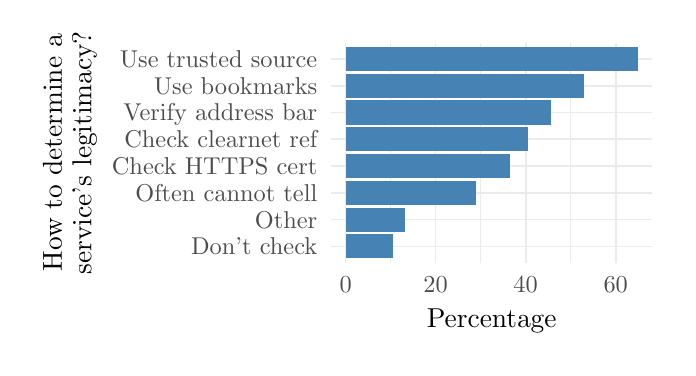
\begin{tikzpicture}[x=1pt,y=1pt]
\definecolor{fillColor}{RGB}{255,255,255}
\path[use as bounding box,fill=fillColor,fill opacity=0.00] (0,0) rectangle (231.26,115.63);
\begin{scope}
\path[clip] (109.60, 30.77) rectangle (225.76,110.13);
\definecolor{drawColor}{gray}{0.92}

\path[draw=drawColor,line width= 0.3pt,line join=round] (131.15, 30.77) --
	(131.15,110.13);

\path[draw=drawColor,line width= 0.3pt,line join=round] (163.68, 30.77) --
	(163.68,110.13);

\path[draw=drawColor,line width= 0.3pt,line join=round] (196.21, 30.77) --
	(196.21,110.13);

\path[draw=drawColor,line width= 0.6pt,line join=round] (109.60, 36.58) --
	(225.76, 36.58);

\path[draw=drawColor,line width= 0.6pt,line join=round] (109.60, 46.26) --
	(225.76, 46.26);

\path[draw=drawColor,line width= 0.6pt,line join=round] (109.60, 55.94) --
	(225.76, 55.94);

\path[draw=drawColor,line width= 0.6pt,line join=round] (109.60, 65.61) --
	(225.76, 65.61);

\path[draw=drawColor,line width= 0.6pt,line join=round] (109.60, 75.29) --
	(225.76, 75.29);

\path[draw=drawColor,line width= 0.6pt,line join=round] (109.60, 84.97) --
	(225.76, 84.97);

\path[draw=drawColor,line width= 0.6pt,line join=round] (109.60, 94.65) --
	(225.76, 94.65);

\path[draw=drawColor,line width= 0.6pt,line join=round] (109.60,104.33) --
	(225.76,104.33);

\path[draw=drawColor,line width= 0.6pt,line join=round] (114.88, 30.77) --
	(114.88,110.13);

\path[draw=drawColor,line width= 0.6pt,line join=round] (147.41, 30.77) --
	(147.41,110.13);

\path[draw=drawColor,line width= 0.6pt,line join=round] (179.95, 30.77) --
	(179.95,110.13);

\path[draw=drawColor,line width= 0.6pt,line join=round] (212.48, 30.77) --
	(212.48,110.13);
\definecolor{fillColor}{RGB}{70,130,180}

\path[fill=fillColor] (114.88, 32.22) rectangle (131.91, 40.93);

\path[fill=fillColor] (114.88, 41.90) rectangle (136.32, 50.61);

\path[fill=fillColor] (114.88, 51.58) rectangle (162.17, 60.29);

\path[fill=fillColor] (114.88, 61.26) rectangle (174.14, 69.97);

\path[fill=fillColor] (114.88, 70.94) rectangle (180.76, 79.65);

\path[fill=fillColor] (114.88, 80.61) rectangle (188.96, 89.32);

\path[fill=fillColor] (114.88, 90.29) rectangle (200.95, 99.00);

\path[fill=fillColor] (114.88, 99.97) rectangle (220.48,108.68);
\end{scope}
\begin{scope}
\path[clip] (  0.00,  0.00) rectangle (231.26,115.63);
\definecolor{drawColor}{gray}{0.30}

\node[text=drawColor,anchor=base east,inner sep=0pt, outer sep=0pt, scale=  0.88] at (104.65, 33.55) {Don't check};

\node[text=drawColor,anchor=base east,inner sep=0pt, outer sep=0pt, scale=  0.88] at (104.65, 43.23) {Other};

\node[text=drawColor,anchor=base east,inner sep=0pt, outer sep=0pt, scale=  0.88] at (104.65, 52.91) {Often cannot tell};

\node[text=drawColor,anchor=base east,inner sep=0pt, outer sep=0pt, scale=  0.88] at (104.65, 62.58) {Check HTTPS cert};

\node[text=drawColor,anchor=base east,inner sep=0pt, outer sep=0pt, scale=  0.88] at (104.65, 72.26) {Check clearnet ref};

\node[text=drawColor,anchor=base east,inner sep=0pt, outer sep=0pt, scale=  0.88] at (104.65, 81.94) {Verify address bar};

\node[text=drawColor,anchor=base east,inner sep=0pt, outer sep=0pt, scale=  0.88] at (104.65, 91.62) {Use bookmarks};

\node[text=drawColor,anchor=base east,inner sep=0pt, outer sep=0pt, scale=  0.88] at (104.65,101.29) {Use trusted source};
\end{scope}
\begin{scope}
\path[clip] (  0.00,  0.00) rectangle (231.26,115.63);
\definecolor{drawColor}{gray}{0.30}

\node[text=drawColor,anchor=base,inner sep=0pt, outer sep=0pt, scale=  0.88] at (114.88, 19.76) {0};

\node[text=drawColor,anchor=base,inner sep=0pt, outer sep=0pt, scale=  0.88] at (147.41, 19.76) {20};

\node[text=drawColor,anchor=base,inner sep=0pt, outer sep=0pt, scale=  0.88] at (179.95, 19.76) {40};

\node[text=drawColor,anchor=base,inner sep=0pt, outer sep=0pt, scale=  0.88] at (212.48, 19.76) {60};
\end{scope}
\begin{scope}
\path[clip] (  0.00,  0.00) rectangle (231.26,115.63);
\definecolor{drawColor}{RGB}{0,0,0}

\node[text=drawColor,anchor=base,inner sep=0pt, outer sep=0pt, scale=  0.99] at (167.68,  7.44) {Percentage};
\end{scope}
\begin{scope}
\path[clip] (  0.00,  0.00) rectangle (231.26,115.63);
\definecolor{drawColor}{RGB}{0,0,0}

\node[text=drawColor,rotate= 90.00,anchor=base,inner sep=0pt, outer sep=0pt, scale=  0.99] at ( 12.32, 70.45) {How to determine a};

\node[text=drawColor,rotate= 90.00,anchor=base,inner sep=0pt, outer sep=0pt, scale=  0.99] at ( 23.01, 70.45) {service's legitimacy?};
\end{scope}
\end{tikzpicture}

    \caption{How our respondents determine an onion service's legitimacy.}
    \label{fig:determining-legitimacy}
\end{figure}

More than half either consult trusted sources (\eg friends or another web site)
or use bookmarks when revisiting onion services.  Many respondents also verify
the domain in the browser's address bar (46\%), check if the corresponding web
site has a link to its onion site (41\%), or hope that the onion service has an
HTTPS certificate (36\%).\footnote{DigiCert is issuing EV-certificates for onion
sites~\cite{DigiCert2015a} but adoption has been slow---presumably in part
because EV certificates require the CA to verify the applicant's identity
and they are not for free.}  Alarmingly, almost 30\% of respondents stated that
they sometimes cannot tell the difference between an authentic service and an
impersonation, and 11\% never check a service's legitimacy in the first place.
People who selected ``Other'' provided a wide variety of ad-hoc phishing
protections---some clearly misguided, which reinforces the scope of the problem.

Originally meant to improve usability, vanity onion domains also play a role in
the context of phishing.  There is concern that the short and recognizable
prefixes tempt users to only verify the prefix and ignore subsequent
characters~\cite{Winter2015a}.  This oversight may allow attackers to create
impersonation domains that feature the prefix but differ in subsequent
characters.  Nurmi~\cite{Nurmi2015a} and Monteiro~\cite{Monteiro2016a} have both
documented such an attack but its effectiveness is not known.

The majority of our respondents appreciates vanity domains because they are easy
to remember (64\%), easy to recognize (64\%), and they provide a unique
``branding'' (34\%).  Some responses indicate that a vanity prefix conveniently
informs about an onion service's topic, letting visitors know what to expect.
Only 8\% dislike vanity onion domains and 15\% don't have an opinion.
Interestingly, some respondents consider vanity domains unfair because wealthy
entities can afford to generate longer prefixes.  Several respondents voiced
their concern that vanity domains create a false sense of security and
facilitate phishing attacks.  In a separate question we inquired how many
characters our respondents verify in onion domains.  43\% verify 13--16 digits,
\ie (almost) the full domain, while 46\% verify up to nine digits, which is
within the realm of brute force attacks.  Finally, a handful number of
respondents cited misguided reasons why they dislike vanity domains, \eg some
believe that vanity domains are a sign of weak hash functions while others
believe that vanity domains make the onion service ``less hidden'' or allow
somebody to create ``the same private key.''

\subsubsection{Perceived security}

Questions 6.4 and 6.6 asked how safe our respondents feel when using Tor Browser
and onion services, respectively.  Figure~\ref{fig:perceived-security} shows the
results.  Using Tor Browser makes 86\% of our respondents feel at least somewhat
safe.  The same is true for 67\% when using onion services---clearly not as many
as for Tor Browser.

\begin{figure}[t]
    \centering
    % Created by tikzDevice version 0.10.1 on 2018-01-12 16:35:49
% !TEX encoding = UTF-8 Unicode
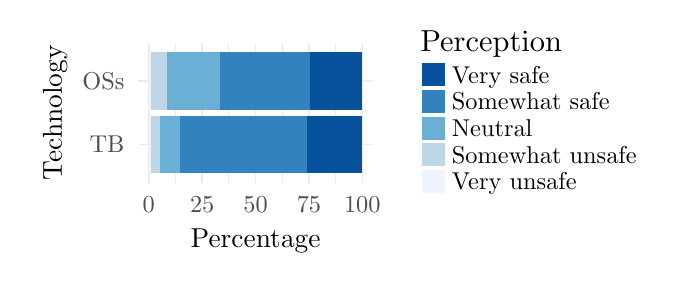
\begin{tikzpicture}[x=1pt,y=1pt]
\definecolor{fillColor}{RGB}{255,255,255}
\path[use as bounding box,fill=fillColor,fill opacity=0.00] (0,0) rectangle (231.26, 86.72);
\begin{scope}
\path[clip] ( 39.91, 30.77) rectangle (124.79, 81.22);
\definecolor{drawColor}{gray}{0.92}

\path[draw=drawColor,line width= 0.3pt,line join=round] ( 53.42, 30.77) --
	( 53.42, 81.22);

\path[draw=drawColor,line width= 0.3pt,line join=round] ( 72.71, 30.77) --
	( 72.71, 81.22);

\path[draw=drawColor,line width= 0.3pt,line join=round] ( 92.00, 30.77) --
	( 92.00, 81.22);

\path[draw=drawColor,line width= 0.3pt,line join=round] (111.29, 30.77) --
	(111.29, 81.22);

\path[draw=drawColor,line width= 0.6pt,line join=round] ( 39.91, 44.53) --
	(124.79, 44.53);

\path[draw=drawColor,line width= 0.6pt,line join=round] ( 39.91, 67.46) --
	(124.79, 67.46);

\path[draw=drawColor,line width= 0.6pt,line join=round] ( 43.77, 30.77) --
	( 43.77, 81.22);

\path[draw=drawColor,line width= 0.6pt,line join=round] ( 63.06, 30.77) --
	( 63.06, 81.22);

\path[draw=drawColor,line width= 0.6pt,line join=round] ( 82.35, 30.77) --
	( 82.35, 81.22);

\path[draw=drawColor,line width= 0.6pt,line join=round] (101.64, 30.77) --
	(101.64, 81.22);

\path[draw=drawColor,line width= 0.6pt,line join=round] (120.93, 30.77) --
	(120.93, 81.22);
\definecolor{fillColor}{RGB}{239,243,255}

\path[fill=fillColor] ( 43.77, 34.21) rectangle ( 44.51, 54.85);
\definecolor{fillColor}{RGB}{189,215,231}

\path[fill=fillColor] ( 44.51, 34.21) rectangle ( 47.92, 54.85);
\definecolor{fillColor}{RGB}{107,174,214}

\path[fill=fillColor] ( 47.92, 34.21) rectangle ( 54.90, 54.85);
\definecolor{fillColor}{RGB}{49,130,189}

\path[fill=fillColor] ( 54.90, 34.21) rectangle (100.90, 54.85);
\definecolor{fillColor}{RGB}{8,81,156}

\path[fill=fillColor] (100.90, 34.21) rectangle (120.93, 54.85);
\definecolor{fillColor}{RGB}{239,243,255}

\path[fill=fillColor] ( 43.77, 57.15) rectangle ( 44.67, 77.78);
\definecolor{fillColor}{RGB}{189,215,231}

\path[fill=fillColor] ( 44.67, 57.15) rectangle ( 50.19, 77.78);
\definecolor{fillColor}{RGB}{107,174,214}

\path[fill=fillColor] ( 50.19, 57.15) rectangle ( 69.60, 77.78);
\definecolor{fillColor}{RGB}{49,130,189}

\path[fill=fillColor] ( 69.60, 57.15) rectangle (101.98, 77.78);
\definecolor{fillColor}{RGB}{8,81,156}

\path[fill=fillColor] (101.98, 57.15) rectangle (120.93, 77.78);
\end{scope}
\begin{scope}
\path[clip] (  0.00,  0.00) rectangle (231.26, 86.72);
\definecolor{drawColor}{gray}{0.30}

\node[text=drawColor,anchor=base east,inner sep=0pt, outer sep=0pt, scale=  0.88] at ( 34.96, 41.50) {TB};

\node[text=drawColor,anchor=base east,inner sep=0pt, outer sep=0pt, scale=  0.88] at ( 34.96, 64.43) {OSs};
\end{scope}
\begin{scope}
\path[clip] (  0.00,  0.00) rectangle (231.26, 86.72);
\definecolor{drawColor}{gray}{0.30}

\node[text=drawColor,anchor=base,inner sep=0pt, outer sep=0pt, scale=  0.88] at ( 43.77, 19.76) {0};

\node[text=drawColor,anchor=base,inner sep=0pt, outer sep=0pt, scale=  0.88] at ( 63.06, 19.76) {25};

\node[text=drawColor,anchor=base,inner sep=0pt, outer sep=0pt, scale=  0.88] at ( 82.35, 19.76) {50};

\node[text=drawColor,anchor=base,inner sep=0pt, outer sep=0pt, scale=  0.88] at (101.64, 19.76) {75};

\node[text=drawColor,anchor=base,inner sep=0pt, outer sep=0pt, scale=  0.88] at (120.93, 19.76) {100};
\end{scope}
\begin{scope}
\path[clip] (  0.00,  0.00) rectangle (231.26, 86.72);
\definecolor{drawColor}{RGB}{0,0,0}

\node[text=drawColor,anchor=base,inner sep=0pt, outer sep=0pt, scale=  0.99] at ( 82.35,  7.44) {Percentage};
\end{scope}
\begin{scope}
\path[clip] (  0.00,  0.00) rectangle (231.26, 86.72);
\definecolor{drawColor}{RGB}{0,0,0}

\node[text=drawColor,rotate= 90.00,anchor=base,inner sep=0pt, outer sep=0pt, scale=  0.99] at ( 12.32, 56.00) {Technology};
\end{scope}
\begin{scope}
\path[clip] (  0.00,  0.00) rectangle (231.26, 86.72);
\definecolor{drawColor}{RGB}{0,0,0}

\node[text=drawColor,anchor=base west,inner sep=0pt, outer sep=0pt, scale=  1.10] at (141.86, 78.11) {Perception};
\end{scope}
\begin{scope}
\path[clip] (  0.00,  0.00) rectangle (231.26, 86.72);
\definecolor{fillColor}{RGB}{8,81,156}

\path[fill=fillColor] (142.58, 65.57) rectangle (150.79, 73.78);
\end{scope}
\begin{scope}
\path[clip] (  0.00,  0.00) rectangle (231.26, 86.72);
\definecolor{fillColor}{RGB}{49,130,189}

\path[fill=fillColor] (142.58, 55.93) rectangle (150.79, 64.15);
\end{scope}
\begin{scope}
\path[clip] (  0.00,  0.00) rectangle (231.26, 86.72);
\definecolor{fillColor}{RGB}{107,174,214}

\path[fill=fillColor] (142.58, 46.30) rectangle (150.79, 54.51);
\end{scope}
\begin{scope}
\path[clip] (  0.00,  0.00) rectangle (231.26, 86.72);
\definecolor{fillColor}{RGB}{189,215,231}

\path[fill=fillColor] (142.58, 36.66) rectangle (150.79, 44.87);
\end{scope}
\begin{scope}
\path[clip] (  0.00,  0.00) rectangle (231.26, 86.72);
\definecolor{fillColor}{RGB}{239,243,255}

\path[fill=fillColor] (142.58, 27.03) rectangle (150.79, 35.24);
\end{scope}
\begin{scope}
\path[clip] (  0.00,  0.00) rectangle (231.26, 86.72);
\definecolor{drawColor}{RGB}{0,0,0}

\node[text=drawColor,anchor=base west,inner sep=0pt, outer sep=0pt, scale=  0.88] at (153.31, 66.65) {Very safe};
\end{scope}
\begin{scope}
\path[clip] (  0.00,  0.00) rectangle (231.26, 86.72);
\definecolor{drawColor}{RGB}{0,0,0}

\node[text=drawColor,anchor=base west,inner sep=0pt, outer sep=0pt, scale=  0.88] at (153.31, 57.01) {Somewhat safe};
\end{scope}
\begin{scope}
\path[clip] (  0.00,  0.00) rectangle (231.26, 86.72);
\definecolor{drawColor}{RGB}{0,0,0}

\node[text=drawColor,anchor=base west,inner sep=0pt, outer sep=0pt, scale=  0.88] at (153.31, 47.37) {Neutral};
\end{scope}
\begin{scope}
\path[clip] (  0.00,  0.00) rectangle (231.26, 86.72);
\definecolor{drawColor}{RGB}{0,0,0}

\node[text=drawColor,anchor=base west,inner sep=0pt, outer sep=0pt, scale=  0.88] at (153.31, 37.74) {Somewhat unsafe};
\end{scope}
\begin{scope}
\path[clip] (  0.00,  0.00) rectangle (231.26, 86.72);
\definecolor{drawColor}{RGB}{0,0,0}

\node[text=drawColor,anchor=base west,inner sep=0pt, outer sep=0pt, scale=  0.88] at (153.31, 28.10) {Very unsafe};
\end{scope}
\end{tikzpicture}

    \caption{The level of security our respondents perceive when using Tor
    Browser (TB) and onion services (OSs).}
    \label{fig:perceived-security}
\end{figure}

Asked about why our respondents feel that way about Tor Browser, our results
reveal that non-experts lack the ability to evaluate (or even understand) Tor's
design which is why they defer to expert opinion, their gut feeling, or the
trust they have in Tor developers.  The Tor Project is perceived to take
security and privacy more seriously than any other browser vendor, which is
appreciated among our respondents.  Most of our respondents' criticism focused
not on Tor Browser but on the underlying Firefox code base.  Many participants
were unhappy with the exploit mitigation techniques, the lack of sandboxing, and
the complex code base.  Chrome was sometimes brought up as the golden standard
for browser security.\footnote{Note that our survey was run before Mozilla
released Firefox Quantum on Nov 14, 2017, which brought substantial improvements
in both security and usability.}  Malicious exit relays were a concern for a
handful of participants while another couple of participants are concerned that
their use of Tor makes them stick out and turn into a target for government
agencies.  Some participants weren't sure if their Tor setup works properly---a
common theme that we also noticed in our interviews: Non-technical users desire
visual feedback confirming that their network traffic comes out ``somewhere
else.''

With respect to onion services, the majority expressed that the added security
and anonymity makes them feel safe.  Another factor contributing to the
perceived security is that onion services make use of far fewer advertising
companies.  Orthogonal to the technology, many participants voiced concern about
illegal and questionable content on onion services, described by some as a
``Wild West.''  Phishing sites, honeypots, and compromised onion sites further
contribute to this perception.


\section{Discussion}
\label{sec:discussion}

We now reflect on our work by elaborating on its shortcomings
(\Cref{sec:biases}) and proposing future research directions
(\Cref{sec:future-work}).

\subsection{Biases}
\label{sec:biases}

A truly uniform sample of Tor users is difficult to obtain.  One strategy would
have been to work with The Tor Project to add a link to our experiment on Tor
Browser's landing page.  While this approach would have reached a large number
of Tor users, we considered it prohibitively invasive.  Besides, people who
rarely restart their Tor Browser or pay no attention to the landing page would
have still missed our experiment.  We therefore decided to ask The Tor Project
to disseminate our survey on its blog and Twitter account.  We believe that this
recruitment strategy was subject to the following biases.

\paragraph{Non-response bias.}
People who noticed our call for volunteers but decided against participating may
have valued their privacy too much, falsely believed that their perspective is
irrelevant, lacked time, or had other reasons not to participate.  Nevertheless,
non-respondents may exhibit traits that are fundamentally different from those
who did participate, which is why their absence in our sample may bias our
results.

\paragraph{Survivor bias.}
We predominantly heard from people who can tolerate Tor's usability issues,
which is why they are still around to tell their tale.  We likely did not hear
from many---if any---people who decided that Tor Browser was not for them, and
were thus unable to tell us what drove them away.  The danger of survivor bias
lies in optimizing the user experience for the subset of people whose tolerance
for inconvenience is higher than the rest.

\paragraph{Self-selection bias.}
Due to the nature of our online survey, participants could voluntarily select
themselves into the group of respondents.  This set of people may be unusually
engaged and technical, which is why they have formed opinions that they
consider worth sharing.  Indeed, the demographic for our online survey in
\Cref{sec:online-survey} was rather young and educated.

\subsection{Future work}
\label{sec:future-work}

The Tor Project is currently working on a security indicator for onion
services~\cite{trac23247}.  \Cref{fig:onion-service} illustrates that Tor
Browser currently, in version 7.0.10, displays an onion service connection like
a plain \textsc{http} connection, thus greatly ``underselling'' the security and
privacy that an onion service connection provides.  The work of Porter Felt
\ea~\cite{Felt2016a} revealed the subtleties that one must consider when
designing security indicators, which highlights the importance of an independent
study of an onion connection security indicator.  Do users correctly understand
the meaning of an onion service indicator?  Do they also understand how it
differs from an \textsc{https} indicator?  Tor Browser's circuit display
\textsc{ui} (see \Cref{fig:tor-button}) is currently experiencing a
redesign~\cite{trac24309}.  Similar to the onion service indicator, an empirical
evaluation of the circuit display could reveal user misunderstandings.  For
example, some users are not familiar with the concept of guard relays and
incorrectly expect each relay in their circuit to change.

Our survey results suggest that there is a need for a system that automates
onion service discovery, \eg, by providing an opt-in mechanism that
automatically publishes onion domains in a public log, allowing users to learn
about new onion domains as they are added to the log.  An orthogonal usability
improvement would be transparent ``upgrading'' from a web site to its
corresponding onion service.  The Tor Project is currently investigating the
problem space on its bug tracker~\cite{trac21952}.  Finally, our survey
responses suggest that there is a need for a privacy-preserving bookmarking tool
that allows users to bookmark sites without leaving a browsing trail on their
hard drives.


\section{Conclusion}
\label{sec:conclusion}

In this work we studied how Tor users interact with onion services and the
broader technology enabling onion services.  Drawing on a mixed-methods
approach, we conducted seventeen semi-structured interviews and collected 828
responses to our online survey.  These two data sets served as the basis of our
analysis and provided unique insight into how Tor users perceive, use, and
understand Tor in general and onion services in particular.

We find that the current state of onion services resembles the web of the 90s.
Pages load slowly, user interfaces are clumsy, and search engines fall short of
expectations.  Users appreciate the extra security, privacy, and NAT punching
properties of onion services, giving rise to numerous use cases, but are
frequently wary of the content that is hosted on them.  Some users found ways to
manage what is perhaps the most striking idiosyncracy of onion services---their
domain format---by using bookmarks, (encrypted) files containing links, and
referring to trusted link aggregators.  Many users however have flawed mental
models of onion services that could increase their susceptibility to phishing
attacks.

Going forward, we believe that research should \first develop a mechanism to
facilitate onion service discovery, \eg, by providing an opt-in mechanism that 
automatically publishes onion service domains; and \second work out how web
sites web sites can redirect Tor users to their respective onion service.
Our code, data, and auxiliary resources are available on our project page at
\url{https://nymity.ch/onion-services/}.


\section*{Acknowledgements}
We want to thank George Kadianakis for helpful feedback.

We want to thank Laura M. Roberts, Roya Ensafi, Will Scott, and Jens Kubiziel
for help with pre-testing the survey.

Thanks to Katherine Haenschen for helping us improve our method.

Finally, we want to thank the broader Tor community for helpful feedback,
volunteering to interview, and taking our survey.

This research was supported in part by the Center for Information Technology
Policy at Princeton University.  This project was further supported in part by
National Science Foundation Awards CNS-1540055 and CNS-1602399.


\balance

{\footnotesize
\printbibliography}

\appendix

\section{Pre-interview survey}
\label{sec:interview-survey}
We asked potential interview subjects to fill out a short survey (see below)
before we proceeded with selecting our subjects.  This survey allowed us to
select for subjects with the most interesting background.

\begin{enumerate}
    \item What is your name?
    \item What is your email address?
    \item Are you 18 years or older?
        \begin{itemize}[label=$\Circle$]
            \item Yes
            \item No
        \end{itemize}
    \item Have you used Tor Browser in the past?
        \begin{itemize}[label=$\Circle$]
            \item Yes
            \item No
        \end{itemize}
    \item Have you used onion services in the past?
        \begin{itemize}[label=$\Circle$]
            \item Yes
            \item No
        \end{itemize}
    \item How do you rate your knowledge about Internet privacy and security?
        \begin{itemize}[label=$\Circle$]
            \item Not at all knowledgeable
            \item Slightly knowledgeable
            \item Somewhat knowledgeable
            \item Moderately knowledgeable
            \item Extremely knowledgeable
        \end{itemize}
\end{enumerate}

\section{Interview questions}
\label{app:interview-questions}

We started the interview by handing our interviewees the consent form and
explained the purpose of our research to them.

\paragraph{Introductory questions}
\begin{enumerate}
    \item Tell us how often and why you use Tor?
    \item Do you remember the first time you used Tor?
\end{enumerate}

\paragraph{Expectations of privacy}
\begin{enumerate}
    \item What would make you use onion services more? (speed, quality/quantity
        of content, better domain format, popular web sites having onion sites)
    \item Who or what are you trying to protect yourself against when using Tor?
    \item The domain format of onion sites is weird.  How do you deal with that?
    \item Would you like it if Tor Browser automatically redirected you to onion
        sites?  Even if that were the case for all onion sites?
    \item How do you learn about new onion sites?
    \item Do you think phishing is a concern with onion sites?  How do you know
        if an onion site is legitimate?
    \item Assume you use Tor to open \texttt{example.com}.  Who can see what?
        What if you open the corresponding onion site instead?
    \item What are you concerned about when using Tor?
    \item Certain things are hidden from certain entities when you are using
        Tor.  Please explain your beliefs.
    \item Some web sites use ``vanity onion domains.''  Whare are your thoughts
        on that?
    \item Explain in your own words how you believe Tor works.
    \item Is there anything else about the usability of onion services that you
        wish to share?
\end{enumerate}

\section{Survey questions}
This section contains our online survey, consisting of seven sections.  Each
section holds a number of questions and their respective responses.  In the
responses, circles indicate that only one response can be selected while squares
indicate the possibility to select multiple responses.

\subsection{Demographic information}
\begin{enumerate}
    \item What is your gender?
        \begin{itemize}[label=$\Circle$]
            \item Female
            \item Male
            \item Other
        \end{itemize}

    \item What is your age?
        \begin{itemize}[label=$\Circle$]
            \item 18--25 years
            \item 26--35 years
            \item 36--45 years
            \item 46--55 years
            \item 56--65 years
            \item Older than 65 years
        \end{itemize}

    \item What is the highest level of education that you completed?
        \begin{itemize}[label=$\Circle$]
            \item Some education, but no high school diploma or equivalent
            \item High school diploma or equivalent
            \item College or university degree (for example a bachelor's degree)
            \item Post-graduate education (for example a master's or a doctorate degree)
        \end{itemize}

    \item How would you rate your knowledge about Internet privacy and security?
        \begin{itemize}[label=$\Circle$]
            \item No knowledge
            \item Mildly knowledgeable
            \item Moderately knowledgeable
            \item Highly knowledgeable
            \item Expert
        \end{itemize}
\end{enumerate}

\subsection{Tor usage}
\begin{enumerate}
    \item Tor Browser is a web browser---similar to Firefox---that allows you
        to browse the web anonymously. Have you ever used Tor Browser?
        \begin{itemize}[label=$\Circle$]
            \item Yes
            \item No
        \end{itemize}

    \item How frequently do you use Tor Browser?\\(Please select the answer
        that applies the most.)
        \begin{itemize}[label=$\Circle$]
            \item Never
            \item On average less than once a month
            \item On average about once a month
            \item On average about once a week
            \item On average about once a day
            \item Tor Browser is my main browser
        \end{itemize}

    \item When using Tor Browser, who do you want to protect your browsing
        activity from?\\(Check all that apply.)
        \begin{itemize}[label=$\Square$]
            \item My government
            \item Other governments
            \item My Internet service provider (ISP)
            \item My school
            \item My employer
            \item Friends and family
            \item Advertising companies
            \item Hackers in open WiFis (for example in coffee shops)
            \item Other (Please elaborate below.)
        \end{itemize}

    \item For quality purposes, please select only ``iPhone'' and ``Android''
        in the options below.
        \begin{itemize}[label=$\Square$]
            \item PC
            \item Mac
            \item iPhone
            \item Android
            \item Other (Please elaborate below.)
        \end{itemize}
\end{enumerate}

\subsection{Onion site usage}
\begin{enumerate}
    \item The Tor Browser allows you to browse ``onion sites.'' Onion sites are
        web sites that can only be accessed over the Tor network. The domains of
        onion sites end with \texttt{.onion} instead of \texttt{.com},
        \texttt{.net}, etc.; they are of constant length; and they tend to
        ``look random.'' For example, The Tor Project's web site,
        \texttt{torproject.org}, is also available at
        \texttt{expyuzz4wqqyqhjn.onion} as an onion site.

    \item How frequently do you use Tor Browser to browse onion sites?\\(Please
        select the answer that applies the most.)
        \begin{itemize}[label=$\Circle$]
            \item I have never used onion sites
            \item On average less than once a month
            \item On average about once a month
            \item On average about once a week
            \item On average about once a day
        \end{itemize}

    \item How frequently do you use onion sites for purposes other than web
        browsing? For example for remote login (SSH) or chat (IRC, or XMPP)?
        \begin{itemize}[label=$\Circle$]
            \item Never
            \item On average less than once a month
            \item On average about once a month
            \item On average about once a week
            \item On average about once a day
        \end{itemize}

    \item Why do you browse onion sites?\\(Check all that apply.)
        \begin{itemize}[label=$\Square$]
            \item Because of the additional anonymity -- traffic to onion sites
                never leaves the Tor network
            \item Because of the additional security -- onion sites provide
                end-to-end security
            \item Some sites I like are only available as onion sites and not
                as normal web sites
            \item No particular reason; I occasionally just click on links to
                onion sites
            \item I read about the ``dark web'' and wanted to form my own
                opinion
            \item Other (Please elaborate below.)
        \end{itemize}

    \item How do you discover new onion sites?\\(Check all that apply.)
        \begin{itemize}[label=$\Square$]
            \item I browse the list of onion site search engines such as
                \texttt{ahmia.fi}
            \item From social networking sites such as Reddit or Twitter
            \item Recommendations from friends and family
            \item I randomly encounter them while browsing the web
            \item I am not interested in learning about new onion sites
            \item Other (Please elaborate below.)
        \end{itemize}

    \item Are you satisfied with the way you discover new onion sites?\\(Check
        all that apply.)
        \begin{itemize}[label=$\Circle$]
            \item Yes
            \item No (Please elaborate below.)
        \end{itemize}

    \item Many people memorize popular domains such as \texttt{youtube.com} and
        \texttt{wikipedia.com} for quick access. How do you deal with the domain
        of onion sites such as \texttt{expyuzz4wqqyqhjn.onion}?\\(Check all that
        apply.)
        \begin{itemize}[label=$\Square$]
            \item I save a list of onion domains in a file on my computer
            \item I write onion domains down using pen and paper
            \item I bookmark onion domains in Tor Browser
            \item I use a web-based bookmarking service such as Firefox Sync or
                Google Bookmarks
            \item I use a search engine each time (for example, to search for
                ``facebook onion site'')
            \item I go to web pages I trust that have links to onion sites
            \item I memorize some onion domains
            \item I don't have a good solution
            \item Other (Please elaborate below.)
        \end{itemize}

    \item The Tor Project is currently working on the next generation of onion
        services. The new onion domain format will consist of 52 characters,
        for example:
        \texttt{a1uik0w1gmfq3i5ievxdm9ceu27e88g6o7pe0rffdw9jmn\-twkdsd.onion}
        Do you expect this to change your browsing habits?
        \begin{itemize}[label=$\Circle$]
            \item Yes (Please elaborate below.)
            \item No (Please elaborate below.)
        \end{itemize}

    \item Do you have a Facebook account?
        \begin{itemize}[label=$\Circle$]
            \item Yes
            \item No
        \end{itemize}

    \item Have you ever logged in to Facebook over its onion site
        \texttt{facebookcorewwwi.onion}?
        \begin{itemize}[label=$\Circle$]
            \item Yes, that is the only way I log in to Facebook
            \item Yes, occasionally
            \item No, never
            \item I didn't know about this onion site until now
        \end{itemize}

    \item For quality purposes, please select ``Yes, more than once'' in the
        options below.
        \begin{itemize}[label=$\Circle$]
            \item Yes, once
            \item Yes, more than once
            \item No
        \end{itemize}

    \item How many onion domains do you have fully memorized?
        \begin{itemize}[label=$\Circle$]
            \item None
            \item One
            \item Two
            \item Three
            \item Four
            \item More than four
        \end{itemize}

    \item Is \texttt{facebookcorewwwi.onion} among the sites that you have
        memorized?
        \begin{itemize}[label=$\Circle$]
            \item Yes
            \item No
        \end{itemize}

    \item Why do you memorize onion domains?\\(Check all that apply.)
        \begin{itemize}[label=$\Square$]
            \item It allows me to open the site more quickly
            \item I don't want to leave any digital traces of the onion sites I
                visit
            \item That way I can be sure that I end up at the right onion site
                and not a phishing site
            \item After typing a domain many times, I automatically start to
                memorize it
            \item Other (Please elaborate below.)
        \end{itemize}

    \item Imagine you had to memorize onion domains. Please rate the difficulty
        of memorizing the following domains.
        \begin{itemize}
            \item \texttt{facebookcorewwwi.onion}
            \item \texttt{expyuzz4wqqyqhjn.onion}
            \item \texttt{torproz4wqqyqhjn.onion}
            \item \texttt{torprojectqyqhjn.onion}
        \end{itemize}
        For each answer, we provided the following Likert scale:
        \begin{itemize}
            \item Very easy
            \item Somewhat easy
            \item Neither easy nor difficult
            \item Somewhat difficult
            \item Very difficult
        \end{itemize}

    \item Please explain the reason for the rating you gave above.

    \item If popular web sites such as YouTube, Twitter, or Amazon offered
        onion sites in parallel to their normal web sites, which one would you
        prefer?
        \begin{itemize}[label=$\Circle$]
            \item Always the normal web site
            \item Always the onion site
            \item Other (Please elaborate below.)
        \end{itemize}

    \item Please explain the reason for the choice you made above.

    \item If Tor Browser could automatically redirect you from a web site to
        its corresponding onion site (for example from \texttt{facebook.com} to
        \texttt{facebookcorewwwi.onion}), would you use this feature?
        \begin{itemize}[label=$\Circle$]
            \item No, never
            \item Yes, for some sites
            \item Yes, always
            \item Other (Please elaborate below.)
        \end{itemize}

    \item Please explain the reason for the choice you made above.

    \item Please rate how important the following criteria are for the
        usability of onion sites.\\(Check all that apply.)
        \begin{itemize}
            \item Page load time
            \item Quality of content (e.g., up-to-date, interesting sites)
            \item Diversity of content (e.g., sites about politics, technology, social media, etc.)
            \item Easy-to-remember domain format
            \item Having an onion service version of popular services such as Facebook
            \item Existence of a search engine (like Google) for onion services
        \end{itemize}
        For each answer, we provided the following Likert scale:
        \begin{itemize}
            \item Very unimportant
            \item Somewhat unimportant
            \item Neutral
            \item Somewhat important
            \item Very important
        \end{itemize}
\end{enumerate}

\subsection{Onion site operation}
\begin{enumerate}
    \item Have you ever set up your own onion site?
        \begin{itemize}[label=$\Circle$]
            \item Yes
            \item No, but I have considered doing it
            \item No, and I have not considered it
        \end{itemize}

    \item Did you experience any issues while setting up your onion site?
        \begin{itemize}[label=$\Circle$]
            \item No
            \item Yes (Please elaborate below.)
        \end{itemize}

    \item Why did you set up your own onion site?\\(Check all that apply.)
        \begin{itemize}[label=$\Square$]
            \item I wanted my site to be anonymous
            \item I wanted my site to have end-to-end security
            \item I used a tool that automatically creates onion sites (for
                example OnionShare or Ricochet)
            \item To make my site accessible behind a NAT device
            \item Out of curiosity
            \item Other (Please elaborate below.)
        \end{itemize}

    \item Were the onion site(s) you set up intended for the general public, or
        only for private use?\\(Check all that apply.)
        \begin{itemize}[label=$\Square$]
            \item For public use (for example, a public blog)
            \item For private use (for example, sharing pictures with a friend)
        \end{itemize}

    \item Please rate the level of concern you would have for the following
        scenarios.
        \begin{itemize}
            \item Somebody deanonymizing my onion service
            \item Somebody taking my onion service offline
            \item Somebody setting up a phishing site targeting my onion service
        \end{itemize}
        For each answer, we provided the following Likert scale:
        \begin{itemize}
            \item Not at all concerned
            \item Slightly concerned
            \item Somewhat concerned
            \item Moderately concerned
            \item Extremely concerned
        \end{itemize}
\end{enumerate}

\subsection{Onion site phishing and impersonation}
\begin{enumerate}
    \item Did you ever type an onion domain manually?
        \begin{itemize}[label=$\Circle$]
            \item Yes
            \item No
        \end{itemize}

    \item Please elaborate on why you typed an onion domain manually?

    \item How do you realize that you made a typo when typing an onion
        URL?\\(Check all that apply.)
        \begin{itemize}[label=$\Square$]
            \item When the page won't load
            \item When a wrong page shows up
            \item I don't know
            \item Other (Please elaborate below.)
        \end{itemize}

    \item Have you ever thought about whether the onion site you are browsing
        is the authentic site you are trying to reach?
        \begin{itemize}[label=$\Circle$]
            \item Yes
            \item No
        \end{itemize}

    \item How do you know an onion site is the legitimate site you are trying
        to reach, and not an impersonation?\\(Check all that apply.)
        \begin{itemize}[label=$\Square$]
            \item I verify (part of) the onion domain in Tor Browser's address
                bar
            \item I use bookmarks when accessing onion sites
            \item I go to the corresponding web site and look for the link to
                its onion site
            \item Sometimes I cannot tell the difference between the legitimate
                and the impersonation site
            \item I copy\&paste onion domains from a trusted source
            \item I check if the onion site's HTTPS certificate is valid (if it
                has one)
            \item I don't check
            \item Other (Please elaborate below.)
        \end{itemize}

    \item How many characters of a domain do you verify? Recall that an onion
        domain has 16 characters.
        \begin{itemize}[label=$\Circle$]
            \item 1--3
            \item 4--6
            \item 7--9
            \item 10--12
            \item 13--16
        \end{itemize}

    \item For quality purposes, please select ``Less than once a month'' in the
        options below.
        \begin{itemize}[label=$\Circle$]
            \item Less than once a month
            \item About once a month
            \item About once a week
            \item About once a day
        \end{itemize}

    \item Have you ever sent Bitcoins to a Bitcoin address that you got from an
        onion site?
        \begin{itemize}[label=$\Circle$]
            \item Yes
            \item No
        \end{itemize}

    \item Some onion site owners use tools to have a short word at the
        beginning of their onion domain. This is why Facebook's domain
        (\texttt{facebookcorewwwi.onion}) looks the way it does. We call these
        customized domains ``vanity onion domains.''

    \item What is your overall opinion on vanity onion domains?\\(Check all
        that apply.)
        \begin{itemize}[label=$\Square$]
            \item I find them useful because they are easier to memorize
            \item I find them useful because they are easier to recognize
            \item I like them because they make an onion site look ``unique''
            \item I dislike them because onion sites shouldn't contain their
                name in their domain
            \item I don't see a benefit
            \item I don't have an opinion
            \item Other (Please elaborate below.)
        \end{itemize}
\end{enumerate}

\subsection{Expectations of privacy}
\begin{enumerate}
    \item Let us move away from onion services and turn to expectations of
        privacy. If you use Tor Browser to open \texttt{http://example.com}, who
        do you believe can see your connection to
        \texttt{http://example.com}?\\(Check all that apply.)
        \begin{itemize}[label=$\Square$]
            \item Your Internet service provider (ISP)
            \item The ISP of \texttt{example.com}
            \item Your Tor ``exit relay''
            \item Your Tor ``guard relay''
            \item Nobody
            \item I don't know
            \item Other (Please elaborate below.)
        \end{itemize}

    \item Now imagine that you are instead using Tor Browser to open the
        \emph{onion site} of \texttt{http://example.com}. Who do you believe can
        see your connection to this onion site?\\(Check all that apply.)
        \begin{itemize}[label=$\Square$]
            \item Your Internet service provider (ISP)
            \item The ISP of the onion site
            \item Your Tor ``exit relay''
            \item Your Tor ``guard relay''
            \item The ``guard relay'' of the onion site
            \item Nobody
            \item I don't know
            \item Other (Please elaborate below.)
        \end{itemize}

    \item How safe do you feel when using Tor Browser compared to another
        browser?
        \begin{itemize}[label=$\Circle$]
            \item Very unsafe
            \item Somewhat unsafe
            \item Neutral
            \item Somewhat safe
            \item Very safe
        \end{itemize}

    \item Please elaborate on why you feel that way when using Tor Browser.

    \item Please tell us about how safe you feel when browing onion sites as
        compared to normal web sites?
        \begin{itemize}[label=$\Circle$]
            \item Very unsafe
            \item Somewhat unsafe
            \item Neutral
            \item Somewhat safe
            \item Very safe
        \end{itemize}

    \item Please elaborate on why you feel that way when using onion sites.

    \item For quality purposes, please select only ``Very unsafe'' in the options
        below.
        \begin{itemize}[label=$\Circle$]
            \item Very unsafe
            \item Somewhat unsafe
            \item Neutral
            \item Somewhat safe
            \item Very safe
        \end{itemize}

    \item Assume you just set up your own onion site. Who do you believe can
        see that this onion site was set up?\\(Check all that apply.)
        \begin{itemize}[label=$\Square$]
            \item The onion site's ISP
            \item The developers of The Tor Project
            \item (Some) Tor relays
            \item Nobody
            \item I don't know
            \item Other (Please elaborate below.)
        \end{itemize}

    \item Facebook already runs the onion site \texttt{facebookcorewwwi.onion}.
        How difficult or easy do you believe is it for someone to create domains
        that begin with the following characters? Note that the {\color{red}
        \texttt{X}} symbols below
        are just placeholders. What matters is the first characters.
        \begin{itemize}
            \item \texttt{facebookcore\textcolor{red}{XXXX}.onion}
            \item \texttt{facebook\textcolor{red}{XXXXXXXX}.onion}
            \item \texttt{face\textcolor{red}{XXXXXXXXXXXX}.onion}
        \end{itemize}
        For each answer, we provided the following Likert scale:
        \begin{itemize}
            \item Very easy
            \item Moderately easy
            \item Neither easy nor difficult
            \item Moderately difficult
            \item Very difficult
            \item I don't know
        \end{itemize}
\end{enumerate}

\subsection{End of survey}
\begin{enumerate}
    \item Finally, is there anything else about the usability of Tor or onion
        services that you wish to share with us?
\end{enumerate}

\section{Coding themes}
\label{sec:coding-themes}

\begin{table*}[ht]
	\centering
	\caption{The codewords we developed while coding our interviews, together
	with their respective explanations, and the number of interviewees who
	brought them up.}

	\label{tab:tor-sketches}

	\begin{tabular}{l l r}
	\toprule
	Codeword & Explanation & Occurences \\
	\midrule

	90s-experience & Tor provides a browsing experience akin to the 90s. & 4 \\
	slow-browsing & Browsing the web over Tor feels slow. & 12 \\
	empowerment & Tor equips users with control over their browsing. & 2 \\
	bad-ux & Parts of the user experience are problematic. & 13 \\
	better-security & Browsing the web over Tor is more secure than over a traditional browser. & 5 \\
	feeling-safe & Tor Browser makes its users feel safe. & 12 \\
	security-limits & There are limits to the security Tor Browser provides. & 13 \\
	transparency & Tor Browser shows its users what is happening ``under the hood.'' & 7 \\
	use-cases & Tor Browser has many use cases. & 15 \\
	cultural-exchange & Tor Browser facilitates cultural exchange. & 1 \\
	desired-features & Users wish for a variety of additional features. & 11 \\
	privacy-expectations & Users have specific expectations of privacy. & 7 \\
	trust & Users place trust in The Tor Project. & 8 \\
	onion-discovery & Users discover onion services in different ways. & 10 \\
	stick-out & The use of Tor can make people ``stick out'' more. & 8 \\
	sensitive-comms & Users consider some types of communication sensitive. & 11 \\
	reputation & The Tor Project has a public reputation. & 4 \\
	worries & Some aspects of using Tor Browser makes users worry. & 9 \\
	domain-format & The onion domain format breaks away from traditional domains. & 9 \\
	unsolved-needs & Users have unsolved needs when they use Tor Browser. & 4 \\
	integration & How well does Tor Browser integrate into users' daily work flow? & 2 \\
	consistency & The browsing experience over Tor is not consistent. & 1 \\
	conflation & Users occasionally conflate concepts. & 6 \\
	targeted-use & Users may use Tor Browser only in specific situations. & 3 \\
	privacy-usability-tradeoff & Users believe there is a trade-off between privacy and usability. & 3 \\
	walk-through & Tor's documentation should walk users through use cases. & 2 \\

	\bottomrule
	\end{tabular}
\end{table*}


\end{document}
